\documentclass{article}

% if you need to pass options to natbib, use, e.g.:
%     \PassOptionsToPackage{numbers, compress}{natbib}
% before loading neurips_2026

% The authors should use one of these tracks.
% Before accepting by the NeurIPS conference, select one of the options below.
% 0. "default" for submission

% the "default" option is equal to the "main" option, which is used for the Main Track with double-blind reviewing.
% 1. "main" option is used for the Main Track
%  \usepackage[main]{neurips_2026}
% 2. "position" option is used for the Position Paper Track
%  \usepackage[position]{neurips_2026}
% 3. "eandd" option is used for the Evaluations & Datasets Track
 % \usepackage[eandd]{neurips_2026}
 % if you need to opt-in for a single-blind submission in the E&D track:
 %\usepackage[eandd, nonanonymous]{neurips_2026}
% 4. "creativeai" option is used for the Creative AI Track
%  \usepackage[creativeai]{neurips_2026}
% 5. "sglblindworkshop" option is used for the Workshop with single-blind reviewing
 % \usepackage[sglblindworkshop]{neurips_2026}
% 6. "dblblindworkshop" option is used for the Workshop with double-blind reviewing
%  \usepackage[dblblindworkshop]{neurips_2026}

% After being accepted, the authors should add "final" behind the track to compile a camera-ready version.
% 1. Main Track
 % \usepackage[main, final]{neurips_2026}
% 2. Position Paper Track
%  \usepackage[position, final]{neurips_2026}
% 3. Evaluations & Datasets Track
 % \usepackage[eandd, final]{neurips_2026}
% 4. Creative AI Track
%  \usepackage[creativeai, final]{neurips_2026}
% 5. Workshop with single-blind reviewing
%  \usepackage[sglblindworkshop, final]{neurips_2026}
% 6. Workshop with double-blind reviewing
%  \usepackage[dblblindworkshop, final]{neurips_2026}
% Note. For the workshop paper template, both \title{} and \workshoptitle{} are required, with the former indicating the paper title shown in the title and the latter indicating the workshop title displayed in the footnote.
% For workshops (5., 6.), the authors should add the name of the workshop, "\workshoptitle" command is used to set the workshop title.
% \workshoptitle{WORKSHOP TITLE}

% "preprint" option is used for arXiv or other preprint submissions
 % \usepackage[preprint]{neurips_2026}

% to avoid loading the natbib package, add option nonatbib:
%    % The original manuscript used the NeurIPS 2026 style file, but that file is not included here.
% Use the standard article class so the document can compile in this workspace.

\usepackage[utf8]{inputenc} % allow utf-8 input
\usepackage[T1]{fontenc}    % use 8-bit T1 fonts
\usepackage{hyperref}       % hyperlinks
\usepackage{url}            % simple URL typesetting
\usepackage{booktabs}       % professional-quality tables
\usepackage{amsfonts}       % blackboard math symbols
\usepackage{nicefrac}       % compact symbols for 1/2, etc.
\usepackage{microtype}      % microtypography
\usepackage[x11names]{xcolor}         % colors
\usepackage{tikz}

%%  Extra packages  %%
\usepackage{amsmath,amsthm,epsfig,amssymb,amsbsy,mathrsfs,mathtools}
\usepackage{enumerate}
\usepackage{bbm}
\usepackage{dsfont}
\usepackage{algorithm}
\usepackage{adjustbox}
\usepackage{subcaption}
\usepackage{algorithm}
\usepackage{algpseudocode}

\usepackage{multirow,makecell}

\usetikzlibrary{arrows.meta}


\usepackage{crossreftools}
\usepackage[capitalize,noabbrev]{cleveref}
\pdfstringdefDisableCommands{%
    \let\Cref\crtCref
    \let\cref\crtcref
}
% \usepackage[square,numbers]{natbib}
\usepackage[giveninits=true,maxbibnames=9, maxcitenames=2, backend=biber]{biblatex}
\addbibresource{references.bib}
\DeclareMathOperator*{\minimize}{minimize}
\DeclareMathOperator*{\argmin}{arg\,min}
\newcommand{\dist}{\operatorname{dist}}
\newtheorem{assumption}{Assumption}
\newtheorem{example}{Example}
\IfFileExists{preamble.tex}{\input{preamble.tex}}{}

% Note. For the workshop paper template, both \title{} and \workshoptitle{} are required, with the former indicating the paper title shown in the title and the latter indicating the workshop title displayed in the footnote. 
\title{$\mathcal{P}$Torch: Narrowing the Gap Between Projection and Gradient--Based Learning}


% The \author macro works with any number of authors. There are two commands
% used to separate the names and addresses of multiple authors: \And and \AND.
%
% Using \And between authors leaves it to LaTeX to determine where to break the
% lines. Using \AND forces a line break at that point. So, if LaTeX puts 3 of 4
% authors names on the first line, and the last on the second line, try using
% \AND instead of \And before the third author name.



\author{%
  David S.~Hippocampus\thanks{Use footnote for providing further information
    about author (webpage, alternative address)---\emph{not} for acknowledging
    funding agencies.} \\
  Department of Computer Science\\
  Cranberry-Lemon University\\
  Pittsburgh, PA 15213 \\
  \texttt{hippo@cs.cranberry-lemon.edu} \\
  % examples of more authors
  % \And
  % Coauthor \\
  % Affiliation \\
  % Address \\
  % \texttt{email} \\
  % \AND
  % Coauthor \\
  % Affiliation \\
  % Address \\
  % \texttt{email} \\
  % \And
  % Coauthor \\
  % Affiliation \\
  % Address \\
  % \texttt{email} \\
  % \And
  % Coauthor \\
  % Affiliation \\
  % Address \\
  % \texttt{email} \\
}


\newcommand{\missingasset}[1]{%
    \fbox{%
        \parbox[c][0.18\textheight][c]{0.9\linewidth}{%
            \centering Missing asset\\[0.35em]\path{#1}%
        }%
    }%
}

\newcommand{\safeinputdiagram}[2]{%
    \IfFileExists{#1.tex}{\resizebox{#2}{!}{\input{#1}}}{\missingasset{#1.tex}}%
}

\newcommand{\safeincludegraphics}[2][]{%
    \IfFileExists{#2}{\includegraphics[#1]{#2}}{\missingasset{#2}}%
}



\usepackage[most]{tcolorbox}

\providecolor{KUL-BLUE}{RGB}{29, 55, 104}
\providecolor{KUL-RED}{RGB}{170, 30, 30}
\providecolor{KUL-ORANGE}{RGB}{230, 140, 0}

\tcbset{
    basecard/.style={
        enhanced,
        frame hidden,
        sharp corners,
        colback=KUL-BLUE!4!white,
        borderline west={3pt}{0pt}{KUL-BLUE},
        coltitle=KUL-BLUE,
        fonttitle=\bfseries,
        attach title to upper,
        after title={:\ \ },
        left=10pt,
        right=10pt,
        top=8pt,
        bottom=8pt,
        boxsep=0pt,
        width=\textwidth
    },
    researchcard/.style={ basecard },
    shift_card/.style={ basecard },
    projectioncard/.style={ basecard },
    % --- NEW: Reusable Reproducibility Box ---
    reprocard/.style={
        basecard,
        colback=gray!5, 
        borderline west={3pt}{0pt}{KUL-ORANGE}, % Uses your custom orange for contrast
        coltitle=KUL-ORANGE,
        fonttitle=\bfseries
    }
}
\begin{document}

\maketitle

\begin{abstract}
Projection-based optimization offers a gradient-free alternative to conventional gradient-based training, but existing frameworks suffer from high computational and memory costs, poor scaling with depth, and limited integration with modern deep learning infrastructure. We introduce $\mathcal{P}$Torch, a projection-based framework built directly on top of PyTorch's \texttt{autograd} engine, and we improve performance through memory-efficient projections and nonlinear relaxation, making the method competitive with gradient-based baselines on shallow MLPs for MNIST and CIFAR-10. Finally, we prove a vanishing-target theorem showing that the layer-wise learning signal decays with depth, providing a projection-based analogue of the vanishing-gradient problem and clarifying one of the central barriers to scaling these methods.
\end{abstract}

\section{Introduction}
Modern deep learning relies almost exclusively on gradient-based optimization, with gradients computed end-to-end via backpropagation \cite{rumelhart1986learning}. However, this paradigm imposes two structural assumptions: every component of the computational graph must admit a gradient (or a tractable subgradient), and parameter updates must propagate through the chain rule. A further motivation for studying alternative approaches to learning is the risk of paradigm lock-in: the overwhelming focus on gradient-based training may lead the community to overlook other learning frameworks that, given comparable research investment, could ultimately prove competitive or even superior. Many alternative paradigms have been proposed in the literature, ranging from classical proposals such as target propagation \cite{lee2015difference}, the method of auxiliary coordinates \cite{carreira2014distributed} and feedback alignment~\cite{lillicrap2016random}, to more recent schemes like equilibrium propagation \cite{scellier2017equilibrium}, forward-forward training \cite{hinton2022forward} and neuroevolution \cite{such2017deep}. Nevertheless, none of these paradigms have achieved widespread adoption, typically bottlenecked by their heuristic approximations and inability to computationally scale on modern hardware.

A promising, mathematically grounded alternative that has recently gained attention is to recast learning as a feasibility problem \cite{elser2019learning, bergmeister2025projection, elser2026learning}. Instead of minimizing a global loss function $\mathcal{L}$, this approach searches for some point $\tilde{\theta}$ in the intersection of multiple constraint sets. These sets are chosen in a way so that from a feasible point $\tilde{\theta}$, one can derive the parameters $\theta$ of the neural network such that the training data is perfectly interpolated. Conceptually, this paradigm shift takes the form
\begin{tcolorbox}[shift_card]
\[
\minimize_{\theta \in \Theta}\, \mathcal{L}(f(x;\theta), y)
\quad \Longrightarrow \quad
\textnormal{find } \tilde{\theta} \in \bigcap_{i=1}^{m} C_i.
\]\end{tcolorbox}
A rich literature exists to tackle such problems, where projection-based methods are the most well-known. Examples of such methods include, but are not limited to, cyclic projections \cite{gubin1967method}, Bregman projections \cite{bregman1967relaxation}, Dykstra's algorithm \cite{dykstra1983algorithm}, and averaged projections \cite{auslender_thesis}. In the two-set case, Douglas--Rachford splitting \cite{douglas1956numerical,eckstein1992douglas} has been studied extensively and applied across a wide range of problems \cite{bauschke2021douglasrachfordalgorithmsolvingpossibly, lindstrom2020surveyyearsdouglasrachford}. Convergence theory for these projection-based methods has been primarily developed in the convex setting \cite{bauschke1996projection}, and there have been recent advances in the nonconvex setting as well \cite{themelis2020douglas,attouch2013convergence,li2016douglas}.

While these projection-based algorithms are promising, they are currently not competitive with gradient-based methods, even for shallow networks. Moreover, they come at the cost of substantial memory overhead, which prohibits scaling at the hardware level. Further, the frameworks in \cite{elser2019learning,bergmeister2025projection} were developed largely in isolation from modern deep learning toolchains and therefore cannot benefit from the many software optimizations that underpin state-of-the-art libraries such as Torch~\cite{paszke2019pytorchimperativestylehighperformance}. In particular, while PJAX \cite{bergmeister2025projection} is built on top of JAX \cite{jax2018github}, it utilizes only the high-performance tensor computation library while all neural network training logic has been completely redefined within PJAX itself. These limitations naturally lead us to our main research question.

%Concretely, there are currently three major limitations. First, the consensus step, explained in \cref{sec:nn_feas}, requires a duplication of the neural network parameters across all samples in a batch, yielding a severe memory consumption. Second, the graph-propagation scheme of \cite{bergmeister2025projection} requires splitting the computational graph into a bipartite graph for every batch, introducing a per-batch overhead absent from standard training pipelines. Third, the frameworks in \cite{elser2019learning,bergmeister2025projection} were developed largely in isolation from modern deep learning toolchains and therefore cannot benefit from the many software optimizations that underpin state-of-the-art libraries such as Torch \cite{paszke2019pytorchimperativestylehighperformance}. In particular, while PJAX \cite{bergmeister2025projection} is built on JAX \cite{jax2018github}, it utilizes only the high-performance tensor computation library while all neural network training logic has been completely redefined within PJAX itself. These identified limitations naturally lead us to our research question.

%Recent work by Bergmeister \cite{bergmeister2025projection} and Elser \cite{elser2019learning} has shown that projection-based algorithms can train neural networks in practice, but at the cost of substantial memory overhead and with empirical performance that remains well below that of gradient-based training. A closer examination reveals three recurring bottlenecks. First, memory consumption is severe: the consensus step in the linear layer scales with $O(N_{\mathrm{in}}N_{\mathrm{out}}B)$ rendering training infeasible on commonly available hardware. Second, the graph-propagation scheme of~\cite{bergmeister2025projection} requires splitting the computational graph into a bipartite graph for every batch, introducing a per-batch overhead absent from standard training pipelines. Third, convergence is noticeably slower than Adam, even on small MLPs. Moreover, these frameworks were developed largely in isolation from modern deep learning toolchains and therefore cannot benefit from the many software optimizations that underpin state-of-the-art libraries such as Torch \cite{paszke2019pytorchimperativestylehighperformance}.\footnote{While PJAX is built on JAX, it utilizes the framework solely as a high-performance tensor computation library; all neural network training logic has been completely redefined within PJAX itself}.

\vspace{0.5em}
\begin{tcolorbox}[researchcard]
Can we design a projection-based training framework native to modern deep learning toolchains that eliminates severe memory bottlenecks, avoids computational overhead, and achieves performance competitive with gradient-based methods?
\end{tcolorbox}
\vspace{0.5em}

%In response to these challenges, we introduce $\mathcal{P}$Torch. The compatibility problem is resolved by building on PyTorch, and by performing graph traversal directly through the native \texttt{autograd}. Further, we introduce and motivate various approaches to improve the performance of projection-based method. As a result, the gap between gradient-based and projection-based optimization in our framework reduces, as closely as possible, to the gap between backpropagation and its projection-based counterpart isolating the optimization strategy from implementation artifacts. 


%Making projection-based learning a mainstream paradigm remains a long-term goal; as with gradient-based 
%optimization, the right implementation tricks to train deep networks such as weight-initialization like He initialization \cite{delving} for gradients have yet to be fully worked out.

\paragraph{Contributions} We address these challenges by introducing $\mathcal{P}$Torch. Concretely, our contributions are as follows.
\begin{enumerate}
    \item \textbf{A PyTorch-native projection framework.}
    We establish a conceptual link between cyclic projections, existing projection-based learning algorithms \cite{elser2019learning,bergmeister2025projection}, and computational graph traversal via PyTorch's \texttt{autograd}. Leveraging this connection, we develop a highly extensible, PyTorch-native projection framework that inherently benefits from modern software optimizations. 
    \item \textbf{Eliminating memory overhead and improving performance.} To mitigate memory constraints, we introduce a fused projection strategy that avoids parameter duplications of prior methods \cite{elser2019learning, bergmeister2025projection}. Furthermore, we demonstrate that modern first-order optimizers, such as Adam \cite{kingma2014adam} and Muon \cite{jordan2024muon}, can be utilized as nonlinear relaxation schemes for cyclic projections. This insight yields substantial empirical gains, enabling our framework to match or exceed the performance of gradient-based baselines on shallow networks. 
    \item \textbf{Vanishing targets.}
    We prove that the base cyclic projection algorithm suffers from a problem analogous to vanishing gradients, thereby limiting its algorithmic scalability to deeper networks. Successfully scaling these models presents a clear avenue of future work: discovering the projection-based equivalents of innovative heuristics like He initialization \cite{delving}, batch normalization \cite{ioffe2015batch}, and residual connections \cite{he2016deep}.
\end{enumerate}
   % For the $\ell_2$ norm, we derive a consensus formula that reduces memory complexity from $O(N_{\mathrm{in}}N_{\mathrm{out}}B)$, where $N_{\mathrm{in}}$ and $N_{\mathrm{out}}$ denote the numbers of input and output neurons and $B$ is the batch size, to $\mathcal{O}(N_{\mathrm{in}}B + N_{\mathrm{out}}B + N_{\mathrm{in}}N_{\mathrm{out}})$. For the $\ell_\infty$ norm, we derive a variant that can be solved in $O(N_{\mathrm{out}})$ time, albeit with worse memory complexity. We further show that first-order optimizers such as Adam and Muon can be interpreted as nonlinear relaxation methods for the cyclic projection update rule, yielding consistent and substantial empirical gains.


\section{Neural network training as a feasibility problem} \label{sec:nn_feas}

\subsection{Intuition behind the method}
Conceptually, a neural network can be viewed as a sequence of interlocking constraints. Each layer imposes a precise mathematical relationship: its output must equal a transformation of its inputs. The overall goal of training is for the network to interpolate or approximate a target dataset. By fixing the network inputs to the data and the outputs to the ground-truth labels, we impose global boundary conditions that generally violate the network's internal constraints. Training therefore amounts to iteratively resolving these local inconsistencies.  Rather than computing global gradients that must be propagated through the chain rule, the algorithm solves a local optimization problem at each layer: 

\textit{What is the minimal adjustment to the local weights, inputs, and outputs needed to exactly re-satisfy the layer constraint?}

By repeatedly applying these local projections from the output back to the input, a learning signal is propagated naturally through the network without requiring gradients.

\subsection{Mathematical description} \label{sec:math_desc}

 %Because this is a novel radient-free paradigm may be unfamiliar in practice, a complete walkthrough is provided in \Cref{app:walk-through}.
We first consider the deterministic case, where we have access to the full dataset $\{(x_1, y_1), \ldots, (x_B, y_B)\}$. Suppose we have a neural network with parameters $\theta^{(1)}, \ldots, \theta^{(N)}$. For ease of presentation, we assume the network has a chain structure, although the extension to more complex topologies is straightforward. In particular, the forward pass for a single sample $(x_b, y_b)$ can be written as
\begin{align*}
    h^{(0)}_b &= x_b \\
    h^{(i+1)}_b &= f_{i+1}(h^{(i)}_b, \theta^{(i+1)}), \quad 
    i=0,\ldots,N-1
\end{align*}
for some functions $f_1, \ldots, f_N$. The output of the network is given by $h^{(N)}$.

\begin{example}
    Let $\theta^i$ be a matrix, $\Sigma$ an activation function and $h_b^{(i-1)}$ a vector. Then $f_i(h^{(i-1)}_b, \theta^{(i)}) = \theta^i h^{(i-1)}_b$ followed by $f_{i+1}(h^{(i)}_b, \theta^{(i+1)}) = \Sigma(h^{(i)}_b)$ is the standard building block of a multilayer perceptron. Note that $\theta^{(i+1)}$ is an ``empty'' variable in this case.
\end{example}
We now proceed to model neural network training as a feasibility problem in a high-dimensional space. Following the framework of \cite{elser2019learning, bergmeister2025projection}, we associate auxiliary variables $\Omega_b =\{h^{(0)}_b, \ldots, h^{(N)}_b, \theta^{(1)}_b, \ldots, \theta_b^{(N)}\}$ with each datapoint $(x_b, y_b)$. Such variables are also introduced in~\cite{carreira2014distributed} where a penalty-based approach is used instead. The feasibility problem consists of finding an $\omega = (\Omega_1, \ldots, \Omega_B)$ in the intersection of some well-chosen constraint sets
\begin{equation} \label{eq:feasibility} \tag{P}
    \textnormal{find } \omega \in \left(\bigcap_{b=1}^B\bigcap_{i=1}^N A_{bi}\right) \bigcap \left(B_{\mathrm{in}} \cap B_{\mathrm{out}}\right) \bigcap \left(\bigcap_{i=1}^N C_i\right).
\end{equation}
For neural network training, there are three types of constraints:
\begin{enumerate}[leftmargin=2em]
    \item \textbf{A}rchitectural constraints: Every layer must satisfy its corresponding input-output transformation. In particular, $\omega \in A_{bi}$ ensures that $h_b^{(i)} = f_i(h_b^{(i-1)}, \theta_b^{(i)})$ for the $b$th datapoint and the $i$th layer.
    \item \textbf{B}atch (data) constraints: The inputs and outputs of the network are fixed to match the current training batch, i.e., $\omega \in B_{\mathrm{in}} \cap B_{\mathrm{out}}$ means that $h_b^{(0)} = x_b$ and $h_b^{(N)} = y_b$ for each $b=1,\ldots,B$.
    \item \textbf{C}onsensus constraints: The duplicated variables must have a single consistent value. Concretely, $\omega \in C_i$ yields $\theta_1^{(i)} = \cdots = \theta_B^{(i)}$ for the $i$th layer. 
\end{enumerate}

If the problem is feasible, then an equivalent minimization problem is
\[
    \omega^\star \in \argmin_{\omega\in\Omega} \underbrace{\frac{1}{2}\left\{\sum_{b=1}^B \sum_{i=1}^N \dist^2(A_{bi}, \omega)   + \dist^2(B_{\mathrm{in}}, \omega) + \dist^2(B_{\mathrm{out}}, \omega) + \sum_{i=1}^N \dist^2(C_i, \omega)\right\}}_{\coloneqq F(\omega)}
\]
where $\dist^2(C, \omega) = \min_{\bar\omega\in C} \|\omega - \bar\omega\|^2$ for a closed set $C$. Indeed, because the squared distance to any set is nonnegative, the global minimum achieves $F(\omega^\star) = 0$ if and only if $\omega^\star$ perfectly satisfies all constraints simultaneously, meaning it lies in the intersection of all defined sets.
\label{sec:feasibility}
\vspace{0.5em}
\begin{tcolorbox}[shift_card]
To summarize, if we find an $\omega$ solving \eqref{eq:feasibility}, then the parameters $\theta^{(1)}, \ldots, \theta^{(N)}$ (which are equal over all datapoints due to the consensus constraint) allow the neural network to perfectly interpolate the data.
\end{tcolorbox}
\vspace{0.5em}

Algorithms to solve feasibility problems utilize projections instead of gradients. In particular, we define the Euclidean projection of $x$ onto a set $C$ by $\Pi_C(\omega) = \argmin_{\bar \omega\in C} \|\omega - \bar\omega\|_2$. This operator is known to be related to the gradient of the squared distance $\dist^2(C,\omega)$. We will later exploit this connection to motivate a nonlinearly relaxed variant of the method we propose.

\begin{example} \label{ex:consensus}
    For the consensus set $C = \{(x_1, \ldots, x_B) : x_1 = \cdots = x_B\}$, we have that $\Pi_C((y_1, \ldots, y_B)) = (\tilde y, \ldots, \tilde y)$ where $\tilde y$ is the average $\frac{1}{B}\sum_{i=1}^B y_i$. Other well-known projections for neural networks can be found in \cref{sec:projections}.
\end{example}

\section{Cyclic projections}
Existing frameworks \cite{elser2019learning,bergmeister2025projection} partition the constraints in \eqref{eq:feasibility} into two disjoint sets and apply the Douglas--Rachford algorithm. This approach has two main limitations. First, making these bipartite projections tractable requires duplicating the network parameters $\theta$ across the batch. This duplication is the root cause of the substantial memory overhead and constitutes a fundamental computational bottleneck to scaling. Second, the computation graph must be bipartitioned. In the current implementation of PJAX, this split is recomputed for each batch, introducing a unnecessary baseline overhead.

To overcome these limitations, we maintain the fine-grained constraint partition defined in \eqref{eq:feasibility} and utilize the method of cyclic projections instead, which successively projects onto each of the sets in a specific cyclic order. We choose an order that corresponds to the PyTorch computational graph: by reinterpreting each functional node in the graph to an associated projection operator, we overwrite the standard backward pass. Consequently, the forward pass remains identical to gradient-based methods, while the backward pass computes a local projection rather than a gradient at each node. The pseudocode for this procedure is detailed in \cref{alg:cyclic}.
\begin{algorithm}
\caption{Cyclic projections method on the PyTorch computational graph.}\label{alg:cyclic}
\begin{algorithmic}[1]
\State $h^{(N)}_b \gets y_b \quad b=1,\ldots, B$  \Comment{Enforce Batch constraint output}
\For{$i=N-1$ \textbf{downto} $0$}\Comment{Traverses the computational graph backwards}
    \For{$b=1$ \textbf{upto} $B$}
        \State $(\bar h^{(i)}_b, \bar \theta^{(i+1)}_b, \bar h^{(i+1)}_b) \in \Pi_{A_{b,i+1}}(h^{(i)}_b, \theta^{(i+1)}_b, h^{(i+1)}_b)$  
        \State $(h^{(i)}_b, \theta^{(i+1)}_b, h^{(i+1)}_b) \gets (\bar h^{(i)}_b, \bar \theta^{(i+1)}_b, \bar h^{(i+1)}_b)$ \Comment{Enforce Architectural Constraint}
    \EndFor
    \State $\bar \theta^{(i+1)} \gets \frac{1}{B}\sum_{b=1}^B \theta_{b}^{(i+1)}$
    \State $\theta^{(i+1)}_b \gets \bar \theta^{(i+1) \quad} b=1,\ldots, B$   \Comment{Enforce Consensus Constraint}
\EndFor
\State $h^{(0)}_b \gets x_b \quad b=1,\ldots,B$ \Comment{Enforce Batch constraint input}
\end{algorithmic}
\end{algorithm}

Nevertheless, although the projection-based algorithm is now integrated with the PyTorch toolchain, \Cref{alg:cyclic} still requires duplication of the variables, while also not having performance on par with standard methods on shallow networks. We now describe the key innovations of $\mathcal{P}$Torch to resolve these issues.

%The basic algorithm can be improved in several ways. In particular, we refine its most sensitive components by developing a more efficient matrix-multiplication projection for linear layers (\cref{sec:matmul}), connecting the method to incremental gradients to incorporate Adam and Muon as nonlinear relaxations (\cref{sec:incremental-grad-descent,sec:relaxation}), and adopting the proximal loss step introduced in PJAX~\cite{bergmeister2025projection} (\cref{sec:moreau}).

\subsection{Optimizing the Linear Layer}
The linear layer is a ubiquitous component of modern neural network architectures. However, its associated projection currently represents the primary computational bottleneck in projection-based frameworks. Because optimizing this operation is essential for scalability, we introduce two key innovations. First, we propose a memory-efficient $\ell_2$ projection that resolves the memory constraints of existing tools like PJAX. Second, we introduce an $\ell_\infty$ projection that, despite a higher computational cost, empirically yields better final accuracy.
\label{sec:matmul}
\subsubsection{Fused consensus and bilinear constraint} \label{subsec:fused}
\paragraph{Motivation.}
As discussed previously, in \cite{elser2019learning,bergmeister2025projection}, the duplication of the network parameters per batch is a primary memory bottleneck. A naive implementation requires constructing an $N_{\mathrm{in}} \times N_{\mathrm{out}} \times B$ tensor, where $N_{\mathrm{in}}, N_{\mathrm{out}}$ are the input and output dimensions of the linear layer respectively, and $B$ is the batch size. This $\mathcal{O}(N_{\mathrm{in}}N_{\mathrm{out}}B)$ memory footprint routinely causes out-of-memory errors on standard hardware, that we also empirically observe in \cref{sec:exp-memory-optimizer}. The authors of PJAX \cite{bergmeister2025projection} note: 

\textit{``the high memory demands of the 4-layer CNN necessitated reducing the number of hidden units per layer to 16 to fit within the available 96GB GPU memory''}

By contrast, our benchmarks include a successfully trained CNN with channel widths of 32-64-128. Furthermore, we have successfully run a ResNet-8 model, as well as CNNs with 2,048 filters. However, as with PJAX, these deeper networks currently result in weak convergence due to the vanishing target problem that we describe in \cref{sec:vanishing-target}.
\paragraph{Derivation.}
One iteration of the cyclic projection algorithm applied to $x$ takes the form $(\Pi_{C_1} \circ \Pi_{C_2} \circ \dots \circ \Pi_{C_N})(x)$. Because operator composition is associative, we are free to group projections and evaluate them as a single, unified operator. We leverage this property to calculate the fused projection $\Pi_C \circ \Pi_A$ onto the bilinear constraint set $A$ (encoding one row of a matrix-vector product) and the consensus set $C$ without introducing duplicated variables.

Concretely, for a sample $b$, layer $i$ and output neuron $j$, we denote the $j$th row of $\theta_b^i$ as $\theta^{i}_b[j,:]$, interpreted as a column vector, while the input $h^{i}_{b}$ is also a column vector. The projection onto the bilinear constraint set that encodes $\theta^{i}_b[j,:]^\top h^{i}_{b} = h^{i+1}_{b}[j]$ then requires solving the optimization problem
\[
     \minimize_{\overline{h}^{i+1}_b\in\mathbb{R};\,\overline{h}^i_b,\overline{\theta}_b^i[j,:]\in\mathbb{R}^{N_{\mathrm{in}}}}\; \ \lVert \overline{h}^i_b-h^i_b\rVert^2 + \alpha^2\lVert \overline{\theta}_b^i[j,:]-{\theta}_b^i[j,:]\rVert^2 + \gamma^2\,(\overline{h}^{i+1}_b-h^{i+1}_b)^2 \text{ s.t. } \ \overline{h}^{i+1}_b = \overline{\theta}_b^i[j,:]^\top \overline{h}^i_b
\]
where $\alpha, \gamma$ are hyperparameters that change the weights in the projection. As shown in \cref{sec:proj-mechanics}, Figure \ref{fig:alpha-g-sweep} the solution can be computed based on some scalar $t_{jb}$ that is found through a Newton iteration. The projected weight then takes the form
\[
    \bar\theta^{i}_{b}[j,:] = u_{jb}\,\theta^{i}[j,:] \;+\; v_{jb}\, h^{i}_{b}{}, \qquad \text{where} \quad u_{jb} := \frac{\alpha}{\alpha - t_{jb}^{2}}, \quad v_{jb} := \frac{t_{jb}}{\alpha - t_{jb}^{2}}.
\]
Next, from Example~\ref{ex:consensus}, it follows that the projection onto the consensus set forces all weights to agree by taking the batch average. Therefore,
\[
    \bar\theta^{i}[j,:] \;=\; \frac{1}{B} \sum_{b=1}^{B} \bar\theta^{i}_{b}[j,:] \implies    \frac{1}{B}\!\left[\, \theta^{i}[j,:] \sum_{b=1}^{B} u_{jb} \;+\; \sum_{b=1}^{B} v_{jb}\, h^{i}_{b}{} \right].
\]
By stacking the scalars $u_{jb}$ and $v_{jb}$ into matrices $U, V \in \mathbb{R}^{N_{\mathrm{out}} \times B}$, and stacking the hidden states into $H \in \mathbb{R}^{B \times N_{\mathrm{in}}}$, we can assemble the update across all output rows simultaneously:
\[
    \bar{\Theta} = \frac{1}{B} \left( \Theta \odot (U\mathbf{1}_{B\times N_{\mathrm{in}}}) + V H \right),
\]
where $\odot$ denotes the Hadamard product and $\mathbf{1}_{B\times N_{\mathrm{in}}}$ is a $B\times N_{\mathrm{in}}$ matrix of all ones. The second term is evaluated as a single $N_{\mathrm{out}} \times B$ by $B \times N_{\mathrm{in}}$ matrix multiplication. Because these computations are fused, no three-dimensional intermediate tensor is ever formed. As a result, peak memory usage drops from $O(N_{\mathrm{in}}N_{\mathrm{out}}B)$ to $\mathcal{O}(N_{\mathrm{in}}B + N_{\mathrm{out}}B + N_{\mathrm{in}}N_{\mathrm{out}})$.

\subsubsection{Projection in a different geometry}
Motivated by the fact that Adam \cite{kingma2014adam} can be seen as an approximation of steepest descent with respect to the $\ell_\infty$-norm  \cite{xie2024implicit} and the recent popular optimizer Muon \cite{jordan2024muon} is related to steepest descent under the spectral norm, we also propose an $\ell_\infty$ variant of the projection onto the bilinear constraint set. The local optimization objective then takes the form
\begin{equation}
\label{eq:bilinf-proj-bilinear-layer}
\min_{\bar{h} \in \mathbb{R}^{N_{\mathrm{in}}}, \bar{\theta} \in \mathbb{R}^{N_{\mathrm{out}} \times N_{\mathrm{in}}}, \bar{h}^+ \in \mathbb{R}^{N_{\mathrm{out}}}} \| (\bar{h}, \bar{\theta}, \gamma^2 \bar{h}^+) - (h, \theta, \gamma^2 h^+) \|_\infty \quad \text{s.t.} \quad \bar{\theta} \bar{h} = \bar{h}^+
\end{equation}
where $\gamma$ is again a hyperparameter to have some more control in the projection.

While this formulation improves final model accuracy, it comes with a computational trade-off. Because the $\ell_\infty$ update depends non-linearly on the absolute values of individual sample-neuron pairs, it cannot be cleanly factored across the batch dimension like the $\ell_2$ case. Consequently, it retains the heavier $\mathcal{O}(N_{\mathrm{in}}N_{\mathrm{out}}B)$ memory footprint.%, though it is more amenable to efficient approximations.

A naive approach to solve \eqref{eq:bilinf-proj-bilinear-layer} requires a sorting procedure, incurring an $\mathcal{O}(N_{\mathrm{in}} \log N_{\mathrm{in}})$ computational bottleneck. To overcome this limitation, we exploit a $45^\circ$ coordinate rotation to develop an $\mathcal{O}(N_{\mathrm{in}})$ branch-masking Newton solver that computes the exact projection in a single pass, completely bypassing the need for sorting. The full derivation of this solver is given in \cref{sec:linf}.

\subsubsection{Choosing the appropriate geometry}
This section highlights a trade-off: we introduce one layer that performs better empirically and another that is more memory efficient, but not one that achieves both simultaneously. Although this hybrid design is conceptually inelegant, there is no practical reason not to mix and match projections. In particular, we can use the memory-efficient projections for large layers with substantial parameter sharing, where memory usage is the primary bottleneck, and use the $\ell_\infty$ projection for all other layers. This strategy allows us to train arbitrary networks while balancing performance and memory efficiency.
%Moreover, solving Equation~\ref{eq:bilinf-proj-bilinear-layer} naively requires sorting $\mathcal{O}(N_{\mathrm{in}})$ kink points for each neuron, leading to an $\mathcal{O}(N_{\mathrm{in}} \log N_{\mathrm{in}})$ computational bottleneck. To overcome this, we exploit a $45^\circ$ coordinate rotation. This allows us to encode the distinct geometric projection regimes into a single, branch-free  mask. By doing so, we 
\subsection{Non-linear Relaxation}
\label{sec:relaxation}
A final key innovation that significantly increases performance rests on the observation that whenever the projection $\Pi_{C}$ is single-valued, $\dist^2(C, \cdot)$ is differentiable with gradient
\[
    \nabla_x \dist^2(C, x) = x - \Pi_C(x).
\] 
Consequently, the cyclic projection algorithm can be viewed as taking incremental-gradient steps~\cite{bertsekas1997nonlinear} on the finite-sum objective $F(\omega)$ detailed in \cref{sec:math_desc}. Unlike standard methods that rely on backpropagating a global loss gradient, this approach utilizes local gradients involving only a small subset of variables (discussed further in \cref{sec:incremental-grad-descent}). Building on this interpretation, it is a natural extension to employ incremental-\textit{optimizer} steps, substituting the standard gradient descent update with any generic first-order optimizer. 

Because $\mathcal{P}$Torch already channels projection residuals through PyTorch's \texttt{autograd}, implementing this requires no algorithmic modifications. The residual directly populates the \texttt{.grad} attribute, allowing standard optimizers to be invoked exactly as they are in a conventional training loop. In practice, we apply this scheme to the weight residuals ($\bar{\theta}^{(i+1)}_b - \theta^{(i+1)}_b$) to achieve adaptive learning rate gradient descent on the weights, while treating the hidden-state residuals as standard projections (equivalent to basic gradient descent). Employing distinct optimization strategies for different parameter groups mirrors the combined use of Muon and Adam \cite{jordan2024muon} in standard gradient-based optimization.

\subsection{Extension to Mini-Batches and the Full Algorithm}
To extend our algorithm to mini-batches, we introduce an inner loop that repeats the backward pass $K$ times for each batch. The hyperparameter $K$ determines how strictly the constraints induced by the current mini-batch are enforced before the algorithm proceeds to the next batch.

This creates a natural optimization trade-off. Larger values of $K$ allow the network to satisfy the current batch constraints more closely, but may lead to overfitting or cause training to stall. Conversely, smaller values of $K$ produce noisier, more stochastic dynamics, as the network switches more rapidly between the potentially conflicting constraints imposed by different mini-batches. This yields the algorithm in \cref{alg:minibatch}. We have also incorporated a proximal operator for the output constraint instead of hard projection. A motivation for this change is provided in \cref{sec:moreau}.

\begin{algorithm}[htbp] \label{alg:minibatch}
\caption{Mini-Batch $\mathcal{P}$Torch}
\begin{algorithmic}[1]
\State $h^{(N)}_b \gets \operatorname{prox}_{\lambda \mathcal{L}}\!\left(h^{(N)}_b,\, y_b\right), \quad b=1,\ldots,B$
\For{$k=1$ \textbf{to} $K$} \Comment{Repeat the backward sweep $K$ times}
    \For{$i=N-1$ \textbf{downto} $0$} \Comment{Traverse the computational graph backward}
        \State $(\bar h^{(i)}, \bar \theta^{(i+1)}, \bar h^{(i+1)}) \in \Pi_{A_{i+1}}(h^{(i)}, \theta^{(i+1)}, h^{(i+1)})$ 
        \State $\bigl(h^{(i)},\;\theta^{(i+1)},\;h^{(i+1)}\bigr) \gets \operatorname{Optimizer}\!\left( h^{(i)} - \bar{h}^{(i)},\; \theta^{(i+1)} - \bar\theta^{(i+1)},\; h^{(i+1)} - \bar{h}^{(i+1)}  \right)$
    \EndFor
\EndFor
\State $h^{(0)}_b \gets x_b$ for $b=1,\ldots,B$
\end{algorithmic}
\end{algorithm}

Note that the explicit \texttt{for} loop over individual samples within a batch has been omitted by using fused operations as described in \cref{subsec:fused}.

In the current $\mathcal{P}$Torch library, $K$ is fixed to one. This design choice enables a significantly more elegant
and efficient implementation: larger values of $K$ require additional memory to propagate the
intermediate targets $h^+$ across multiple backward sweeps and necessitate a non-standard training
loop. With $K=1$, the framework is a near drop-in replacement for standard PyTorch.
\section{Vanishing Target Signals in Deep Networks}
\label{sec:vanishing-target}
A fundamental limitation of projection-based algorithms in deep architectures is the attenuation of the learning signal with depth. We formalize this phenomenon below.

At training step $n$, define the \emph{target signal magnitude} at hidden layer $i$ by
\[
\delta^{i} \;:=\; \bigl\|\bar{h}^{i} - h^{i}\bigr\|_2.
\]

\begin{assumption}
\label{ass:non-expansive}
Consider the constraint set associated with layer $i+1$ to be
\[
    A_{i+1} := \{ (h^{(i)}, \theta^{(i+1)}, h^{(i+1)}) \mid h^{(i+1)} = f_{i+1}(h^{(i)}, \theta^{(i+1)}) \}.
\]
Let $x \coloneq (h^{(i)}, \theta^{(i+1)}, h^{(i+1)})$ and $y \coloneq (h^{(i)}, \theta^{(i+1)}, \tilde{h}^{(i+1)})$ be given points. Defining $R \coloneq \|x - y\|_2$, we assume that for all points $\bar{y}$ satisfying $\|x - \bar{y}\|_2 \leq R$, the projection $\Pi_{A_{i+1}}$ satisfies the local non-expansiveness property:
\[
    \|\Pi_{A_{i+1}}(x) - \Pi_{A_{i+1}}(\bar{y})\|_2 \leq \|x - \bar{y}\|_2.
\]
\end{assumption}
In general, (global) nonexpansiveness only holds for projections onto convex sets, see for example \cite[Proposition 4.16]{bauschke2020correction}. Nevertheless, this local assumption is motivated by empirical evidence in \cref{sec:Non-Expansiveness}.

Under Assumption~\ref{ass:non-expansive}, for the cyclic projection algorithm, the target signal magnitude $\delta^{(i),n}$ 
is monotonically non-increasing as targets are propagated backward from the output layer $N$. Formally,
\[
\delta^{(i),n} \;\leq\; \delta^{(i+1),n} \quad \text{for all } 0 \leq i \leq N-1,
\]
with strict inequality whenever $\|\Delta \theta^{(i+1)}\|_2 > 0$, i.e., whenever the 
layer is actively learning. The general statement follows by induction; when every layer 
satisfies $\|\Delta \theta^{(i+1)}\|_2 > 0$, the target magnitudes are strictly 
decreasing across all layers. The full proof is deferred to \cref{sec:proof-vanishing-targets}.
\vspace{0.5em}
\begin{tcolorbox}[shift_card]
Depth Barrier: In a network that is actively learning, cyclic projections result in a diminishing learning signal to early layers. For networks of sufficient depth, the target difference at the earliest layers reaches machine precision, rendering parameter updates in those layers negligible.
\end{tcolorbox}
\vspace{0.5em}

While no definitive solution to this problem has been found, several workarounds have been explored, including skip connections as in PJAX~\cite{bergmeister2025projection} and applying Muon's \cite{jordan2024muon} Newton--Schulz orthogonalization, without rescaling, to the hidden states while using a separate optimizer for the weights (\cref{sec:exp-relaxation-location}, \cref{fig:orthogonalization}). These heuristics substantially improve performance in deeper networks, largely by stabilizing the target differences across layers. However, performance remains significantly weaker than that of traditional gradient-based learning, making this framework impractical for training deep networks at larger scale, and so we focus on smaller-scale experiments in the next section.

% ---------------------------------------------------------------

\section{Experiments}
\label{sec:experiments}
% ---------------------------------------------------------------
We evaluate $\mathcal{P}$Torch against Torch~\cite{paszke2019pytorchimperativestylehighperformance} as a gradient-based reference implementation and the projection-based reference implementation \texttt{pjax}~\cite{bergmeister2025projection}
across fifteen experiments. \cref{sec:exp-mlp}--\cref{sec:exp-cnn}
benchmark end-to-end accuracy on the standard MNIST and CIFAR-10
classification tasks; \cref{sec:arch-init}--\cref{sec:exp-memory-optimizer}
isolate choices specific to $\mathcal{P}$Torch (proximal
loss, efficient matrix-multiplication projection, optimizer choice and
relaxation placement, and projection norm);

\paragraph{Shared protocol.}
Unless explicitly overridden in a per-experiment paragraph, all
benchmarks share the configuration in
\cref{tab:shared-protocol}.

% =========================================================
% Reproducibility Box (Reusable)
% =========================================================

% ---------------------------------------------------------------
\subsection{Shallow MLP: MNIST and CIFAR-10}
\label{sec:exp-mlp}
% ---------------------------------------------------------------
\begin{tcolorbox}[reprocard, title=Setup]
A single-hidden-layer MLP with 512 ReLU units is trained on MNIST
($784 \to 512 \to 10$) and CIFAR-10 ($3072 \to 512 \to 10$). All three
frameworks instantiate this architecture with identical widths, and the optimizers listed in Table~\ref{tab:shared-protocol}.
\end{tcolorbox}

\begin{figure}[ht]
\centering
\begin{minipage}[t]{0.44\textwidth}
    \centering
    \safeincludegraphics[width=\textwidth]{images/mlp/CIFAR10_1L_TIME.png}
\end{minipage}
\hfill
\begin{minipage}[t]{0.44\textwidth}
    \centering
    \safeincludegraphics[width=\textwidth]{images/mlp/MNIST_1L_STEP.pdf}
\end{minipage}
\caption{Single-hidden-layer MLP (width 512): CIFAR-10 validation accuracy vs.\ wall-clock time (left) and MNIST validation accuracy vs.\ optimization step (right). Curves show the mean over three seeds; shaded bands indicate $\pm 1$ standard deviation.}
\label{fig:shallow-mlp}
\end{figure}

\paragraph{Interpretation.}
The purpose of this benchmark is to illustrate both the promise of the method and the broader risk of paradigm lock-in. Projection-based training already yields competitive results on shallow MLPs; with sustained effort comparable to that devoted to gradient-based methods, its performance could improve substantially. Relative to \texttt{pjax}, $\mathcal{P}$Torch achieves significantly better wall-clock performance by leveraging PyTorch's optimized \texttt{autograd} graph traversal together with the more efficient projections described in the previous sections. Compared with Torch using Adam under the shared protocol in \cref{tab:shared-protocol}, a small gap remains during the initial optimization steps.% ---------------------------------------------------------------
\subsection{Vanishing target signal and depth}
\label{sec:exp-vanishing}
% ---------------------------------------------------------------
Two complementary experiments probe the depth barrier predicted in
Section~\ref{sec:vanishing-target}.
\begin{tcolorbox}[reprocard, title=Setup]
\emph{(a) Identity-recovery} We train fully linear MLPs of depth $L \in \{2, 4, 8\}$ and width $32$ to recover the identity map $f(x) = x$ on i.i.d.\ Gaussian inputs $x \sim \mathcal{N}(0, I_{32})$. Each batch contains $16$ samples. We log the per-layer target magnitude $\delta_k^{n} := \frac{\|\bar h^{(k),n} - h^{(k),n}\|_2 }{B}$ at training step $n=1$ and the final training MSE.

\vspace{2.0pt}

\emph{(b) 4-layer MLP classification.} A 4-layer MLP is trained on MNIST and CIFAR-10 with the protocol of Section~\ref{sec:exp-mlp} but for $10{,}000$ steps with \texttt{HardMarginLoss} as the target loss. The same architecture
in \texttt{torch} (Adam, lr $=10^{-3}$, cross-entropy) is the gradient
baseline.
\end{tcolorbox}


\begin{figure}[ht]
\centering
\safeincludegraphics[width=0.9\textwidth]{images/deep/vanishing_combined.pdf}
\caption{
per-layer target signal magnitude $\delta_k^{n}$ at
step~$1$ for varying depths (left) and final training MSE vs.\ depth
(right) on the identity-recovery probe.
}
\label{fig:depth-barrier}
\end{figure}

\paragraph{Interpretation.}
The identity-recovery probe shows that $\delta_k^{n}$ decays  as $k$ moves away from the output, with layers three steps from the output already reaching machine precision. On MNIST and CIFAR-10, the four-layer $\mathcal{P}$Torch MLPs lag far behind their single-hidden-layer counterparts. Both observations are consistent with the theory in \cref{sec:vanishing-target}. Although this is a negative result, it serves an important purpose: it identifies the framework's weak point and clarifies where further progress is needed. We provide an initial step in this direction in \cref{fig:orthogonalization} by applying orthogonalization to the hidden states; although this helps, it does not resolve the underlying issue.

\begin{figure}[ht]
    \centering
    % First independent figure
    \begin{minipage}{0.48\textwidth}
        \vspace{0.5pt}
        \safeincludegraphics[width=\linewidth]{images/deep/deep_mlp_TIME.png}
        \caption{Validation accuracy vs.\ wall-clock time for a
        4-layer MLP on MNIST. The performance gap
        relative to \texttt{torch} widens with depth, consistent with the
        depth-barrier prediction of \cref{sec:vanishing-target}.}
    \end{minipage}\hfill
    % Second independent figure
    \begin{minipage}{0.48\textwidth}
        \centering
        \vfill
        \safeincludegraphics[width=\linewidth]{images/other_benchmarks/CIFAR10_CONV.pdf}
        \caption{Validation accuracy vs.\ wall-clock time on CIFAR-10 with the
        CNN architecture. $\mathcal{P}$Torch convergences and final accuracy lag behind \texttt{Torch}.}
        \label{fig:cnn}
    \end{minipage}
\end{figure}



% ---------------------------------------------------------------
\subsection{Convolutional networks: small CNN on CIFAR-10}
\label{sec:exp-cnn}
% ---------------------------------------------------------------
\begin{tcolorbox}[reprocard, title=Setup]
Given the depth barrier of Section~\ref{sec:vanishing-target}, we do
not attempt to train deep ResNets with $\mathcal{P}$Torch. Instead we
train a 6-layer convolutional network on CIFAR-10: three blocks of with channel widths $\{32, 64, 128\}$  followed by a flatten and a fully connected $\ell_\infty$ classifier head. Training runs for $10{,}000$ steps with batch size~$32$  $\mathcal{P}$Torch uses \texttt{ProjectionAdam} (lr $=10^{-3}$) with the $\ell_2$ matrix projection in convolutional layers
\end{tcolorbox}

\paragraph{Interpretation.}
Effective CNNs typically rely on depth, yet projection-based learning degrades as network depth increases. This mismatch makes training high-performing CNNs challenging. In additional experiments, we trained a ResNet-8, which despite extensive tuning reached only $50\%$ accuracy on CIFAR-10. While these results show that training deeper CNNs is computationally possible with $\mathcal{P}$Torch, they also highlight significant limitations. Substantial progress is still needed before projection-based methods become a practical choice for standard convolutional architectures. 

\section{Beyond $\mathcal{P}$Torch}
$\mathcal{P}$Torch demonstrates that projection-based learning can be competitive with gradient-based methods on shallow architectures. By building natively on PyTorch's autograd engine, it removes prior memory bottlenecks and connects cyclic projections to first-order optimization through nonlinear relaxation.

However, two major obstacles remain. The first is depth: our vanishing-target theorem shows that the learning signal attenuates exponentially with network depth, creating a challenge structurally analogous to the vanishing-gradient problem that limited early deep learning before the advent of residual connections and principled initialization schemes. The second is coverage: effective projections for normalization layers remain unresolved, and a fully projection-based attention mechanism is still blocked by unresolved difficulties surrounding softmax and simplex projections.

Neither barrier is likely to fall in a single paper. Gradient-based deep learning succeeded not because every early idea worked, but because enough ideas were explored for the successful ones to accumulate into a practical toolkit. Projection-based learning may require a similar period of experimentation. In that setting, $\mathcal{P}$Torch provides both a practical research platform and a competitive baseline: its projections can already improve existing systems such as PJAX, while its native integration with PyTorch enables hybrid architectures and direct comparison with standard optimization pipelines.
\printbibliography


\newpage
\appendix
\crefalias{section}{appendix}
\crefalias{subsection}{appendix}

\section{Related Work}

\paragraph{Target propagation.}
Target propagation is a  gradient-free learning paradigm where layer-wise targets are propagated backward through the network instead of gradients \cite{lee2015difference}. While these methods attempt to generate these targets by approximating the inverse of the forward map, our projection-based approach instead treats layer-wise updates as local feasibility problems. Instead of relying on approximate inverses. $\mathcal{P}$torch computes targets by mathematically projecting the current state onto the layer's constraint set to find the absolute smallest adjustment required to satisfy the network's architectural constraints. Despite these different mechanisms for generating local targets, both approaches share a fundamental limitation: the attenuation of the learning signal with depth. 

\paragraph{ADMM-based deep learning.}
The Alternating Direction Method of Multipliers (ADMM)\cite{neal2011distributed} offers a prominent alternative to the projection-based training of neural networks. Similar to projection-based methods, ADMM decouples the network into per-layer subproblems by introducing auxiliary variables and enforcing consistency constraints via a Lagrangian penalty. Wang et al.~\cite{10.1145/3292500.3330936} advanced this line of work with the dlADMM algorithm, which updates parameters in a backward-then-forward sweep to propagate information more efficiently. Crucially, their approach reduces the subproblem complexity from $O(n^3)$ to $O(n^2)$ using iterative quadratic approximations and backtracking, while also establishing rigorous global convergence guarantees under mild conditions on the loss and activation functions. Ultimately, the layer-wise decomposition in dlADMM conceptually aligns with $\mathcal{P}$Torch's target propagation: both methods bypass end-to-end differentiation by decomposing the global objective into isolated, layer-wise optimization steps propagated through the computational graph.

\paragraph{Gradient-free optimization frameworks.}
A variety of other gradient-free optimization methods have been proposed in the literature, including the Method of Auxiliary Coordinates \cite{carreira2014distributed}. By unfolding the network into layers, this approach replaces a complex nested optimization problem with local optimization problems at the level of individual layers. Distinct paradigms such as neuroevolution have also attracted significant attention and even inspired dedicated frameworks \cite{tang2022evojax}. Another notable alternative is the more recent Forward-Forward algorithm \cite{hinton2022forward}. However, a common thread across these approaches is that none has yet achieved widespread adoption in mainstream deep learning.

\section{A Walk Through the backwards pass}
\label{app:walk-through}

This section walks through the cyclic projections algorithm for a single batch. In particular, it shows how the abstract algorithm works in practice and what happens when a \texttt{loss.backward()} call is performed in $\mathcal{P}$Torch.
 
\subsection{Forward and Backward Semantics}
Consider a feedforward network with $N$ layers, with computational graph $\mathcal{G} = (\mathcal{V}, \mathcal{E})$. Each node $v \in \mathcal{V}$ corresponds to a layer function $f_i$ acting on the previous hidden state and (possibly empty) parameters,
\begin{equation}
h^{(i)} \;=\; f_i\bigl(h^{(i-1)}, \theta^{(i)}\bigr), \qquad i = 1, \dots, N,
\end{equation}
with $h^{(0)} = x$ and network output $h^{(N)}$. To exploit the native \texttt{autograd} engine, $\mathcal{P}$Torch redefines the semantics of the forward and backward passes for each node.

For ease of presentation, we suppress the sample index $b$ (Section \ref{alg:cyclic}) throughout this section and assume each projection is a fused operator that calculates the local projection and the consensus sequentially within a single operation.

\subsection{Loss Projection and Target Initialization}
 
\begin{figure}[htbp]
\centering
\resizebox{\textwidth}{!}{%
\input{drawings/init_state_backprop}
}
\caption{Initialization of the backward pass: the network output $h^{(N)}$ is coupled to
the loss constraint via the proximal operator of Section~\ref{sec:moreau}}
\end{figure}

Let $y$ denote the data target for the batch. The backward pass is initialized by the proximal step on the output layer.

The target for the network output $h^{(N)}$ is the proximal step:
\begin{equation}
\label{eq:proximal-step}
h^{(N)} \;=\; \mathrm{prox}_{\lambda \mathcal{L}}\!\bigl(h^{(N)},\, y\bigr) \;\in\; \underset{u}{\mathrm{arg\,min}} \left( \mathcal{L}\bigl(u, y\bigr) + \frac{\lambda}{2} \bigl\|u - h^{(N)}\bigr\|_2^2 \right).
\end{equation}

This $h^{(N)}$ is then propagated to the preceding layer as its target.

 
\subsection{Linear-Layer Update}
\begin{figure}[htbp]
\centering
\resizebox{\textwidth}{!}{%
\providecolor{KUL-BLUE}{RGB}{29, 55, 104}
\providecolor{KUL-ORANGE}{RGB}{230, 140, 0}

\begin{tikzpicture}[
    scale=0.95,
    transform shape,
    font=\small,
    >=stealth,
    op/.style={rectangle, rounded corners=1pt, draw=black!65, fill=black!8, thick, minimum width=2.8cm, minimum height=1.0cm, align=center},
    param/.style={circle, draw=black!65, fill=black!10, text=black, thick, minimum size=1.2cm, inner sep=1pt, align=center},
    state/.style={circle, draw=black!65, fill=black!5, text=black, thick, minimum size=1.0cm, inner sep=1pt, align=center},
    io/.style={circle, draw=black!65, fill=black!5, text=black, thick, minimum size=0.9cm, inner sep=1pt, align=center},
    focusState/.style={circle, draw=KUL-BLUE!85!black, fill=KUL-BLUE!12, thick, minimum size=1.4cm, inner sep=1pt, align=center},
    focusIo/.style={circle, draw=KUL-BLUE!85!black, fill=KUL-BLUE!12, thick, minimum size=0.95cm, inner sep=1pt, align=center},
    focusOp/.style={rectangle, rounded corners=1pt, draw=KUL-ORANGE!85!black, fill=KUL-ORANGE!15, thick, minimum width=3.2cm, minimum height=1.1cm, align=center},
    focusParam/.style={circle, draw=KUL-BLUE!85!black, fill=KUL-BLUE!12, text=black, thick, minimum size=1.2cm, inner sep=1pt, align=center},
    flow/.style={->, thick, black!55},
    active/.style={->, thick, KUL-BLUE!85!black},
    support/.style={->, thick, black!50}
]

    % Inactive layers (Forward pass history)
    \node[state] (h0) at (0,0) {$h^{(0)}$};
    \node[op] (lin1) at (3.5,0) {$\theta^{(1)}h^{(0)}$};
    \node[state] (h1) at (6.5,0) {$h^{(1)}$};
    \node[op] (sig) at (9.5,0) {$\Sigma(h^{(1)})$};

    % Active projection nodes for the output linear layer
    \node[focusState] (h2) at (12.5,0) {$h^{(2)}$};
    \node[focusOp] (lin3) at (16.0,0) {$\theta^{(3)}h^{(2)}$};
    \node[focusIo] (h3) at (19.0,0) {${h}^{(3)}$};

    % Parameters
    \node[param] (w1) at (3.5,2.0) {$\theta^{(1)}$};
    \node[focusParam] (w3) at (16.0,2.0) {$\theta^{(3)}$};

    % Flow connections for the inactive parts
    \draw[flow] (h0) -- (lin1);
    \draw[flow] (lin1) -- (h1);
    \draw[flow] (h1) -- (sig);
    \draw[flow] (sig) -- (h2);

    % Parameter support for inactive layer
    \draw[support] (w1) -- (lin1);

    % Active connections converging on the local projection step
    \draw[active] (h2) -- (lin3);
    \draw[active] (w3) -- (lin3);
    \draw[active] (h3) -- (lin3); % Target flowing backwards into the projection

\end{tikzpicture}
}
\caption{Update of the output linear layer: projection onto the architectural constraint
$A_{N}$ couples the output target ${h}^{(N),n}$ to the deepest hidden state
$h^{(N-1),n}$ and the weights $\theta^{(N),n}$.}
\label{fig:next_back_prop}
\end{figure}

Assume layer $N$ is linear with weights $\theta^{(N)}$, so $f_N\bigl(h^{(N-1)},\theta^{(N)}\bigr) = \theta^{(N)} h^{(N-1)}$. The corresponding architectural constraint set is:
\begin{equation}
A_{N} \;:=\; \bigl\{\bigl(h^{(N-1)},\, \theta^{(N)},\, h^{(N)}\bigr) \,\bigm|\, h^{(N)} = \theta^{(N)} h^{(N-1)} \bigr\}.
\end{equation}
Given the current hidden state and weights, together with the output target, the projection
\begin{equation}
\bigl(\bar{h}^{(N-1)},\; \bar{\theta}^{(N)},\; \bar{h}^{(N)}\bigr) \;\in\; \Pi_{A_{N}}\!\bigl(h^{(N-1)},\; \theta^{(N)},\; h^{(N)}\bigr)
\end{equation}
simultaneously yields the target hidden state $\bar{h}^{(N-1)}$ and the projected weights $\bar{\theta}^{(N)}$, and the adjusted output target $\bar{h}^{(N)}$. Following the nonlinear relaxation strategy, the next parameter iterate is obtained by feeding the projection residual into the chosen first-order optimizer:

\begin{equation}
\bigl(h^{(N-1)},\;\theta^{(N)},\; h^{(N)}\bigr) \gets \operatorname{Optimizer}\!\left( {h}^{(N-1)} - \bar h^{(N-1)},\; {\theta}^{(N)} - \bar \theta^{(N)},\; {h}^{(N)} - \bar h^{(N)} \right)
\end{equation}

with relaxation or step size $\eta$. For the plain projection update, this reduces to $\theta^{(N)} = \bar{\theta}^{(N)}$. The hidden state $h^{(N-1)}$ then becomes the output target passed to the projection $P_{A_{N-1}}$ of the preceding activation function layer.

\subsection{Activation function Update}
\begin{figure}[htbp]
\centering
\resizebox{0.78\textwidth}{!}{%
\providecolor{KUL-BLUE}{RGB}{29, 55, 104}
\providecolor{KUL-ORANGE}{RGB}{230, 140, 0}

\begin{tikzpicture}[
    scale=0.95,
    transform shape,
    font=\small,
    >=stealth,
    op/.style={rectangle, rounded corners=1pt, draw=black!65, fill=black!8, thick, minimum width=2.8cm, minimum height=1.0cm, align=center},
    param/.style={circle, draw=black!65, fill=black!10, text=black, thick, minimum size=1.2cm, inner sep=1pt, align=center},
    state/.style={circle, draw=black!65, fill=black!5, text=black, thick, minimum size=1.0cm, inner sep=1pt, align=center},
    io/.style={circle, draw=black!65, fill=black!5, text=black, thick, minimum size=0.9cm, inner sep=1pt, align=center},
    focusState/.style={circle, draw=KUL-BLUE!85!black, fill=KUL-BLUE!12, thick, minimum size=1.4cm, inner sep=1pt, align=center},
    focusIo/.style={circle, draw=KUL-BLUE!85!black, fill=KUL-BLUE!12, thick, minimum size=0.95cm, inner sep=1pt, align=center},
    focusOp/.style={rectangle, rounded corners=1pt, draw=KUL-ORANGE!85!black, fill=KUL-ORANGE!15, thick, minimum width=3.2cm, minimum height=1.1cm, align=center},
    focusParam/.style={circle, draw=KUL-BLUE!85!black, fill=KUL-BLUE!12, text=black, thick, minimum size=1.2cm, inner sep=1pt, align=center},
    flow/.style={->, thick, black!55},
    active/.style={->, thick, KUL-BLUE!85!black},
    support/.style={->, thick, black!50}
]

    % Inactive layers (Forward pass history)
    \node[state] (h0) at (0,0) {$h^{(0)}$};
    \node[op] (lin1) at (3.5,0) {$\theta^{(1)}h^{(0)}$};
    \node[param] (w1) at (3.5,2.0) {$\theta^{(1)}$};

    % Active projection nodes for the activation layer
    \node[focusState] (h1) at (6.5,0) {$h^{(1)}$};
    \node[focusOp] (sig) at (9.5,0) {$\Sigma(h^{(1)})$};
    \node[focusIo] (h2) at (12.5,0) {${h}^{(2)}$};

    % Flow connections for the inactive parts
    \draw[flow] (h0) -- (lin1);
    \draw[flow] (lin1) -- (h1);

    % Parameter support for inactive layer
    \draw[support] (w1) -- (lin1);

    % Active connections converging on the local projection step
    \draw[active] (h1) -- (sig);
    \draw[active] (h2) -- (sig); % Target flowing backwards into the projection

\end{tikzpicture}
}
\caption{Projection through the activation constraint $A_{N-1}$, which carries no
parameters.}
\label{fig:next_back_prop_mid}
\end{figure}
 
Now consider the preceding activation layer $f_{N-1} = \Sigma$. As $\theta^{(N-1)}$ is empty for activation layers, the architectural constraint reduces to a relation between two hidden states:
\[
A_{N-1} \;:=\; \bigl\{\bigl(h^{(N-2)},\, h^{(N-1)}\bigr) \,\bigm|\,
h^{(N-1)} = \Sigma\bigl(h^{(N-2)}\bigr) \bigr\}.
\]

The projection yields the subsequent updated iterate $h^{(N-1)}$ and the target input $\bar{h}^{(N-2)}$, which becomes the target output for the preceding layer:
\begin{equation}
\bigl(\bar{h}^{(N-2)},\; \bar h^{(N-1)}\bigr) \;\in\; \Pi_{A_{N-1}}\!\bigl(h^{(N-2)},\; h^{(N-1)}\bigr)
\end{equation}

This sequential projection procedure repeats, propagating targets backward through the computational graph $\mathcal{G}$ until the root is reached.

\section{Hybrid architectures}
To demonstrate the flexibility of \texttt{$\mathcal{P}$Torch}, we confirm foundational support for hybrid architectures that interleave projection-based and gradient-based paradigms within a single computational graph. While preliminary testing validates this interoperability.

\section{Practical Considerations for Projection-Based Training}
To make projection-based neural network training more accessible to future researchers, this section discusses implementation and tuning details that help ensure successful experiments.

\subsection{Architecture and Initialization}
\label{sec:arch-init}
When designing architectures for this framework, we recommend shallow networks, as they are both more stable and empirically stronger than deeper alternatives. In addition, ensure that every layer influencing the propagated targets is implemented using $\mathcal{P}$Torch modules. Mixing in standard PyTorch layers (for example, standard linear layers) can interfere with the autograd-based target propagation mechanism, causing targets to be interpreted as gradients, or vice versa. Batch Normalization and similar normalization layers currently degrade performance substantially and should therefore be avoided.

Initialization is also critical. At present, the framework relies on the same initialization schemes commonly used in gradient-based training, but our experiments indicate that initialization has a major effect on both convergence and the final state reached by the network.

\begin{figure}[ht]
\centering
\safeincludegraphics[width=1.0\textwidth]{images/effect_of_init.pdf}
\caption{Impact of initialization strategies on network convergence across varying depths. Training accuracy is shown over 200 steps for networks of depth 2, 4, and 8, comparing three initialization methods: standard normal distribution (std=0.01), He normal, and scaled orthogonal. While all evaluated methods achieve convergence in shallow networks (Depth = 2), the normal distribution initialization degrades significantly as depth increases, failing to converge at Depth = 8. In contrast, He normal and orthogonal initializations maintain stability and enable successful convergence in deeper architectures.}
\label{fig:effect-of-init}
\end{figure}

\subsection{Memory scaling and optimizer choice}
\label{sec:exp-memory-optimizer}
Choosing the optimizer is the most important practical decision in this framework. In most settings, the Muon projection optimizer yields the strongest results and is therefore our recommended default. If faster initial progress is needed, or if Muon diverges, SGD is a robust alternative. Adam is also promising, but it is substantially less stable and often requires learning-rate tuning before it trains reliably. When using SGD or Adadelta, higher learning rates sometimes as large as 10 are best. A practical tuning strategy is to start at 1 and adjust upward or downward depending on training stability. By contrast, Muon and Adam generally perform best at their standard learning rates of $10^{-3}$.

Empirically, both $\mathcal{P}$Torch and \texttt{torch} scale better and have a lower memory baseline than \texttt{pjax}, allowing substantially larger networks to be trained before memory is exhausted. As shown in Figure~\ref{fig:memory}, for a single linear-layer projection, \texttt{pjax} scales as $O(N_{\mathrm{in}}N_{\mathrm{out}}B)$, whereas $\mathcal{P}$Torch reduces this to $\mathcal{O}(N_{\mathrm{in}}B + N_{\mathrm{out}}B + N_{\mathrm{in}}N_{\mathrm{out}})$, matching standard PyTorch's asymptotic scaling. For researchers who are using \texttt{pjax}, we strongly recommend replacing its default matrix-multiplication projection with our $\ell_2$ projection to alleviate these memory bottlenecks. 
\begin{figure}[ht]
\centering
\begin{subfigure}[t]{0.55\textwidth}
    \centering
    \safeincludegraphics[width=\textwidth]{images/memory_vs_k.pdf}
    \caption{Peak memory versus input dimension for a single linear-layer projection. PJAX scales substantially worse than $\mathcal{P}$Torch and \texttt{torch}. For small input dimensions, $\mathcal{P}$Torch uses roughly $10\times$ more memory than \texttt{torch}, but this gap narrows as the input dimension increases. We hypothesize that the remaining increase relative to \texttt{torch} is primarily an implementation artifact.}
    \label{fig:memory}
\end{subfigure}
\hfill
\begin{subfigure}[t]{0.43\textwidth}
    \centering
    \safeincludegraphics[width=\textwidth]{images/optimizer_comparison.pdf}
    \caption{Validation accuracy on MNIST versus optimization step for four
    optimizers applied to updates derived from the $\mathcal{P}$Torch projection
    residual. Curves report the mean over three random seeds.}

    \label{fig:optimizer-comparison}
\end{subfigure}
\label{fig:memory-optimizer}
\end{figure}
\subsection{Projection Mechanics}
\label{sec:proj-mechanics}
The choice of projection norm fundamentally alters training dynamics. The $\ell_\infty$ projection is computationally more expensive but converges faster per optimization step and reaches a higher final accuracy. As the batch size grows, the efficient $\ell_2$ implementation becomes substantially faster per wall-clock time than the $\ell_\infty$ projection. Consequently, with larger batch sizes, it takes longer in wall-clock time for the $\ell_\infty$ curve to overtake the $\ell_2$ baseline.
\begin{figure}[ht]
    \centering
    \begin{subfigure}[t]{0.45\textwidth}
        \centering
        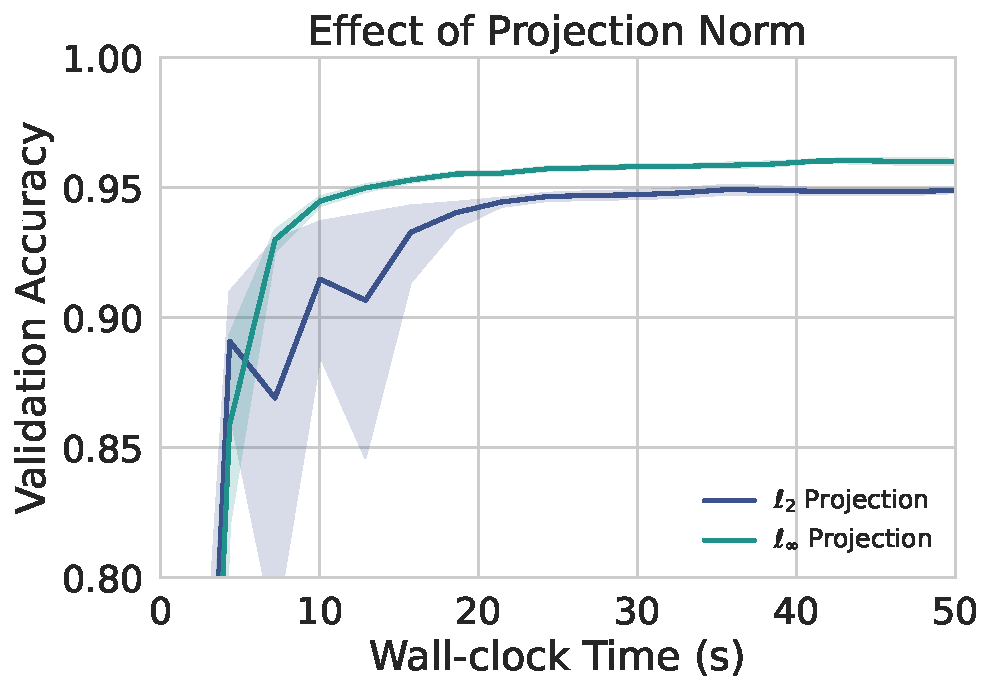
\includegraphics[width=\textwidth]{images/mlp/norm_comparison_time_32.pdf}
        \caption{Batch size 32}
        \label{fig:norm-comparison-32}
    \end{subfigure}
    \hfill
    \begin{subfigure}[t]{0.45\textwidth}
        \centering
        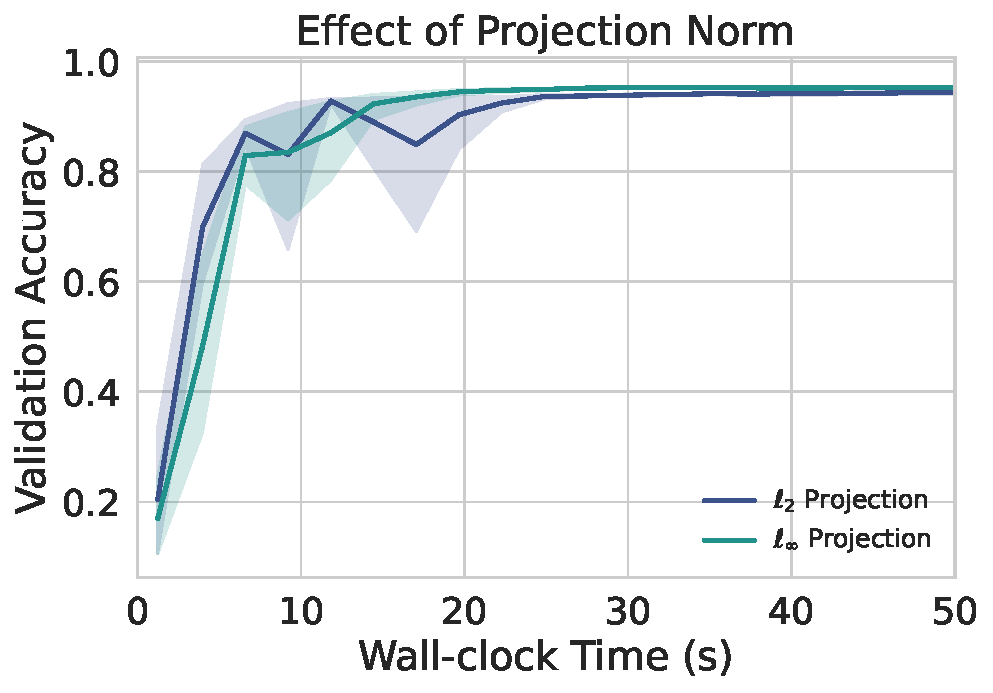
\includegraphics[width=\textwidth]{images/mlp/norm_comparison_time_1024.pdf}
        \caption{Batch size 1024}
        \label{fig:norm-comparison-1024}
    \end{subfigure}
    \caption{Effect of projection norm ($\ell_2$ vs.\ $\ell_\infty$) on validation accuracy over wall-clock time. While $\ell_2$ initially outpaces $\ell_\infty$ in wall-clock time at larger batch sizes due to computational efficiency, $\ell_\infty$ consistently overtakes it to achieve higher final accuracy given sufficient training duration.}
    \label{fig:norm-comparison}
\end{figure}
\label{ef}
The projection behavior can be further tuned via the $\alpha$ and $\gamma$ parameters, which dictate whether the weights or activations absorb the majority of the update. 
Specifically, setting $\gamma \to \infty$ leaves the output values unchanged, whereas setting $\alpha \to  \infty$ leaves the weights unchanged. 
In practice, the framework is highly robust and relatively insensitive to these hyperparameters; however, careful tuning within a reasonable range, typically $[0.01, 500]$, can yield modest gains when maximizing accuracy.\footnote{These hyperparameter sweeps were conducted using WandB and a customized version of PTorch; consequently, we do not provide a replication script. However, both tools are primarily intended as auxiliary components and are straightforward to replicate.}
\begin{figure}[ht]
\centering
\begin{subfigure}[t]{0.48\textwidth}
\centering
\safeincludegraphics[width=\textwidth]{images/alpha_g_sweep.png}
\caption{Hyperparameter sweep illustrating the sensitivity to $\alpha$ and $\gamma$.}
\label{fig:alpha-g-sweep}
\end{subfigure}
\hfill
\begin{subfigure}[t]{0.48\textwidth}
\centering
\safeincludegraphics[width=\textwidth]{images/matmul_projection_sweep_2d.png}
\caption{MatMul projection showing the impact of these parameters on all matrices in a linear node.}
\label{fig:matmul-sweep}
\end{subfigure}
\label{fig:projection-params}
\end{figure}

In the current framework, the number of backward passes is fixed at 1, as this allows for a substantially more efficient and elegant implementation. However, this choice may not be optimal, since using multiple backward passes can improve performance per step
\begin{figure}[ht]
\centering
\safeincludegraphics[width=1\textwidth]{images/other_benchmarks/mnist_cyclic_pure_bp_comparison.pdf}
\caption{Error convergence and validation accuracy as a function of the number of backward passes on the MNIST benchmark.}
\label{fig:backward-passes}
\end{figure}


\subsection{Advanced Relaxations and Loss Formulation}
\label{sec:exp-relaxation-location}
To further stabilize training, first-order relaxations can be applied to the projection residuals. Where this relaxation is applied is critical: applying it (for example, with Adam or Muon) only to the weight residuals performs better than applying it to both weight and hidden-state residuals, or than using no relaxation at all.
To keep the framework simple, we apply relaxation only to the weights by default. However, in some cases, such as the XOR benchmark, applying relaxation more broadly can be beneficial. This remains an underexplored direction.

Finally, regarding the loss formulation, replacing the hard target-assignment with a proximal-loss step (Section \ref{sec:moreau}) accelerates convergence. Similar benefits to softening the loss constraint have also been reported in prior projection-based literature like PJAX \cite{bergmeister2025projection}.

\begin{figure}[ht]
    \centering
    % Left Figure
    \begin{minipage}{0.48\textwidth}
        \centering
        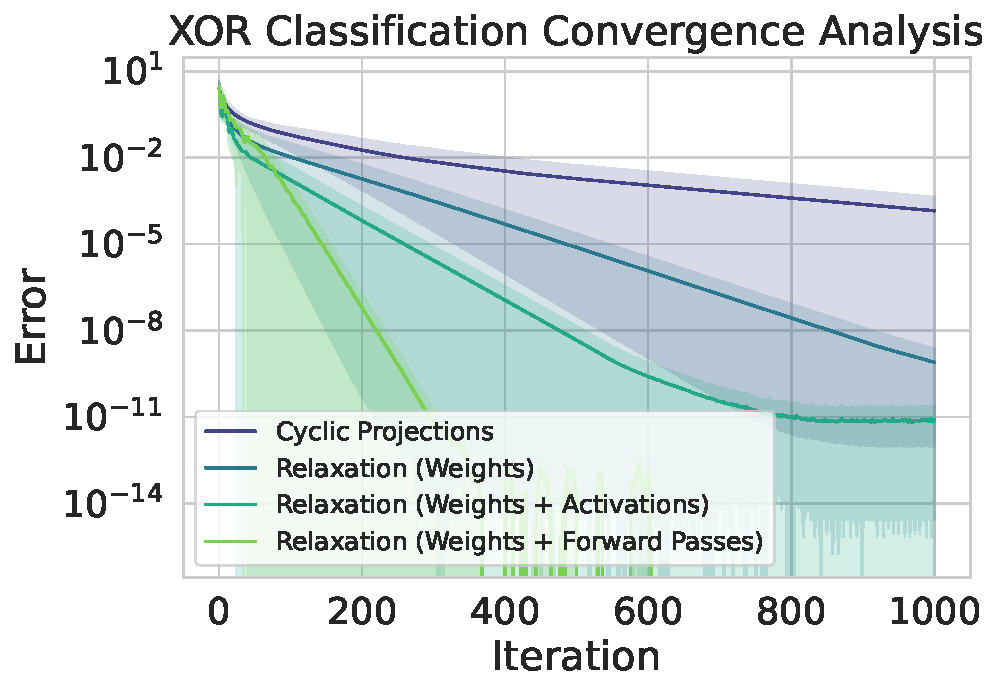
\includegraphics[width=\textwidth]{images/other_benchmarks/xor_activations.pdf}
        \caption{First-order relaxation applied to the hidden states on the xor benchmark.}
        \label{fig:relaxation-location}
    \end{minipage}
    \hfill % Adds horizontal space between the two
    % Right Figure
    \begin{minipage}{0.48\textwidth}
        \centering
        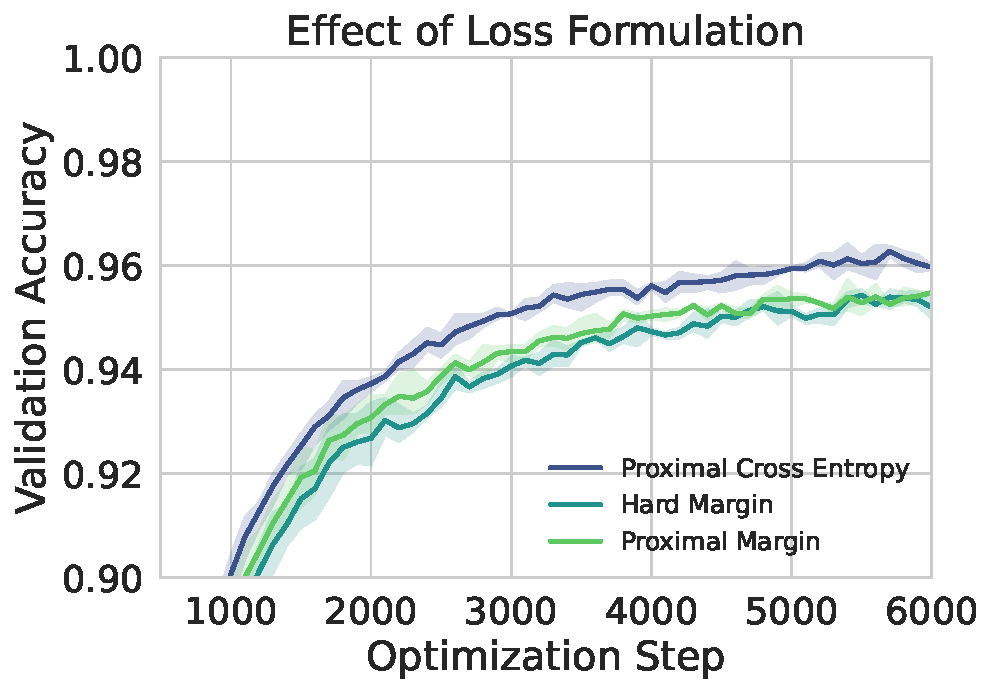
\includegraphics[width=\textwidth]{images/effect_of_loss.pdf}
        \caption{Replacing hard target-assignment with a proximal-loss step of strength $\lambda = 1$ accelerates convergence.}
        \label{fig:effect-of-loss}
    \end{minipage}
\end{figure}

One hidden-state optimization strategy implemented in $\mathcal{P}$Torch applies Muon\cite{jordan2024muon} specifically, the Polar Express orthogonalization\cite{amsel2025polar} \emph{without} the rescaling step to the hidden-state residuals. This stabilizes the target signal as depth increases. Although this treatment causes a small accuracy regression on shallow networks, it benefits deeper networks far more than it harms shallow ones. s 
\begin{figure}[ht]
\centering
\safeincludegraphics[width=\textwidth]{images/deep/vanishing_combined_muon.pdf}
\caption{Applying Newton--Schulz orthogonalization without rescaling on
the hidden-state residuals stabilises $\delta_k^{n}$ across depths, at
the cost of a small accuracy regression on shallow networks. The
treatment helps deeper networks more than it hurts shallow ones.}
\label{fig:orthogonalization}
\end{figure}


\section{Details of the $\mathcal{P}$Torch algorithm}
\subsection{Connection to incremental gradient descent}
\label{sec:incremental-grad-descent}
To motivate the non-linear relaxations (\cref{sec:relaxation}), we make explicit the connection between cyclic projections and the incremental gradient method \cite{bertsekas1997nonlinear}. Recall from \cref{sec:feasibility} that training reduces to the finite-sum problem $F(\omega)$
\[
    \min_{\omega} \; \frac{1}{2}\left\{\sum_{b=1}^{B}\sum_{i=1}^{N} \bigl(\dist^{2}(A_{bi}, \omega) \;+\; \dist^{2}(B_{\mathrm{in}}, \omega) \;+\; \dist^{2}(B_{\mathrm{out}}, \omega) \;+\; \sum_{i=1}^{N} \dist^{2}(C_i, \omega)\bigr)\right\}
    \label{eq:finite_sum}
\]

which has the form $F(\omega) = \sum_{j=1}^{M} f_j(\omega)$, with each component $f_j(\omega) = \dist^{2}(C_j, \omega)$ a squared distance to a constraint set. Wherever the projection $\Pi_{C_j}$ is single-valued, $f_j$ is differentiable with
\begin{equation}
    \nabla f_j(\omega) \;=\; \omega - \Pi_{C_j}(\omega).
    \label{eq:dist_gradient}
\end{equation}

A subtlety is that the constraint sets induced by the network are non-convex, so $P_{C_j}(\omega)$ doesn't need not be unique. At points $\omega$ that are equidistant from two or more elements of $C_j$, the projection is ambiguous and~\eqref{eq:dist_gradient} is not well defined. This issue is benign for two reasons. First, the set of such points has Lebesgue measure zero, so~\eqref{eq:dist_gradient} holds almost everywhere by Rademacher's theorem. Second, on this exceptional set the residual $\omega - P_{C_j}(\omega)$ remains a valid subgradient under any choice of $P_{C_j}(\omega)$, so the update direction is well-defined in either case. The situation is identical to that of $\mathrm{ReLU}$ at the origin: non-differentiable at a single point, yet trained without difficulty using a subgradient selection.

With~\eqref{eq:dist_gradient} in hand, the cyclic projection update of Algorithm~\ref{alg:cyclic} is exactly an incremental gradient step on $F$. The plain projection step
\begin{equation}
    \bar \theta^{i+1} \;\gets\; \Pi_{C_j}\!\bigl(\theta^{i+1}\bigr)
    \label{eq:plain_projection}
\end{equation}
can be rewritten as
\begin{equation} \
    \bar \theta^{(i+1)}\gets\; (1-\alpha)\,\theta^{i+1} \;+\; \alpha\, \Pi_{C_j}\!\bigl(\theta^{i+1}\bigr)
    \qquad \alpha = 1,
    \label{eq:relaxed_projection}
\end{equation}
This is the relaxed projection with relaxation factor $\alpha$. Rearranging~\eqref{eq:relaxed_projection} and substituting~\eqref{eq:dist_gradient} gives
\begin{equation}
    \bar \theta^{i+1} \;\gets\; \theta^{i+1} \;-\; \alpha\bigl(\theta^{i+1} - \Pi_{C_j}(\theta^{i+1})\bigr) \;=\; \theta^{i+1} \;-\; \alpha\,\nabla f_j\!\bigl(\theta^{i+1}\bigr),
    \label{eq:projection_as_gradient_step}
\end{equation}
which is precisely the incremental gradient update~\cite[Eq.~(2.78)]{bertsekas1997nonlinear}
\begin{equation}
    \omega^{k+1} \;=\; \omega^{k} \;-\; \alpha^{k}\,\nabla f_{j_k}(\omega^{k})
    \label{eq:incremental_gradient}
\end{equation}
applied to the finite-sum objective~\eqref{eq:finite_sum}, where the step size is $\alpha^k$ and the index $j_k$ is chosen according to the cyclic order induced by the computational graph. This connection motivates the use of first-order optimizers, since the projection residuals we provide are gradients of the finite-sum problem.
\subsection{Why the proximal loss step helps: a Moreau-envelope view}
\label{sec:moreau}
 
The rigid target-assignment step replaces the network's final prediction
$h^{N}$ with the true target $y$. The proximal-loss variant softens this
by replacing $h^{N}$ with a compromise between staying close to $h^{N}$
and reducing the loss $\mathcal{L}(\cdot,y)$. Concretely, given a
smoothing strength $\lambda>0$, we define
\begin{equation}
\bar h^{N} \;:=\; \arg\min_{u}\;
\underbrace{\mathcal{L}(u,y)}_{\text{loss at }u}
\;+\;
\underbrace{\frac{\lambda}{2}\,\bigl\|u-h^{N}\bigr\|^{2}}_{\text{stay near }h^{N}} ,
\label{eq:prox-def}
\end{equation}
and update $h^{N}\leftarrow\bar h^{N}$. We call $\bar h^{N}$ the
proximal target.
The minimum value attained in~\eqref{eq:prox-def} defines a new function
of $h^{N}$:
\begin{equation}
\mathcal{L}_{\lambda}(h^{N},y)
\;:=\;
\min_{u}\Bigl\{\,\mathcal{L}(u,y)+\tfrac{\lambda}{2}\bigl\|u-h^{N}\bigr\|^{2}\Bigr\}.
\label{eq:env-def}
\end{equation}
This is the Moreau envelope of $\mathcal{L}$ at strength $\lambda$.
It is a smoothed lower bound: $\mathcal{L}_{\lambda}\le\mathcal{L}$ pointwise,
$\mathcal{L}_{\lambda}\to\mathcal{L}$ as $\lambda\to\infty$, and
$\mathcal{L}_{\lambda}$ is differentiable in $h^{N}$ even when
$\mathcal{L}$ is not. A direct calculation gives the gradient in closed form:
\begin{equation}
\nabla_{\!h^{N}}\,\mathcal{L}_{\lambda}(h^{N},y)
\;=\;
\lambda\,\bigl(h^{N}-\bar h^{N}\bigr).
\label{eq:moreau-grad}
\end{equation}
Equation~\eqref{eq:moreau-grad} is the key identity: the displacement
produced by the proximal step, scaled by $\lambda$, \emph{is} the gradient
of the smoothed loss. Consequently, the update $h^{N}\leftarrow\bar h^{N}$
is exactly one gradient-descent step of step size $1/\lambda$ on
$\mathcal{L}_{\lambda}(\cdot,y)$:
\[
h^{N}\;\leftarrow\;\bar h^{N}
\;=\;h^{N}-\tfrac{1}{\lambda}\nabla_{\!h^{N}}\mathcal{L}_{\lambda}(h^{N},y).
\]
 Globally, the proximal-loss variant therefore optimizes the surrogate
\begin{equation}
\widetilde{F}_{\lambda}(\omega)
\;=\;
\Phi_{\mathrm{net}}(\omega)\;+\;\mathcal{L}_{\lambda}\!\bigl(h^{N}(\omega),\,y\bigr),
\end{equation}
where $\Phi_{\mathrm{net}}(\omega)$ collects all internal network terms.
The original (unsmoothed) target-assignment objective is recovered as
$\lambda\to \infty$.

An important property of this is that the optimum is preserved. For convex $\mathcal{L}(\cdot,y)$, $\mathcal{L}_{\lambda}$ and $\mathcal{L}$ share the same set of minimizers for every $\lambda>0$~\cite{rockafellar1998variational}, so choosing $\lambda$ trades smoothness against surrogate tightness without moving the solution.

The empirical gain can be explained by the bounded backward signal: the residual that initiates the backward pass is $\lambda(h^{N}-\bar h^{N})$, which for mean-squared-error loss equals $\frac{\lambda}{1+\lambda}(h^{N}-y)$, i.e.\ the rigid residual $h^{N}-y$ contracted by a factor in $(0,1)$. More generally, whenever $\mathcal{L}(\cdot,y)$ is convex the proximal residual is no larger than the rigid residual, and whenever $\mathcal{L}$ is itself Lipschitz (e.g.\ hinge, Huber) it is bounded uniformly in $h^{N}$ by the Lipschitz constant of $\mathcal{L}$. 

\section{Details of the vanishing targets}
\subsection{Experimental verification of local non-expansiveness}
\label{sec:Non-Expansiveness}
Recall our core assumption regarding the local non-expansiveness of the Matrix Multiplication projection. Consider the architectural constraint set of a linear layer, defined as
\[
    A := \{(X, W, Z) \mid Z = WX\}.
\]
Let $x_0 \coloneq (X_0, W_0, Z_0)$ be a given reference point. We assume that there exists a radius $\varepsilon > 0$ such that for all points $x_1, x_2$ in the closed ball $\mathcal{B}(x_0, \varepsilon)$ centered at $x_0$ (i.e., satisfying $\|x_0 - x_1\| \leq \varepsilon$ and $\|x_0 - x_2\| \leq \varepsilon$), the projection $\Pi_A$ satisfies the local non-expansiveness property:
\[
    \|\Pi_A(x_1) - \Pi_A(x_2)\| \leq \|x_1 - x_2\|.
\]
\begin{figure}[htbp]
    \centering
    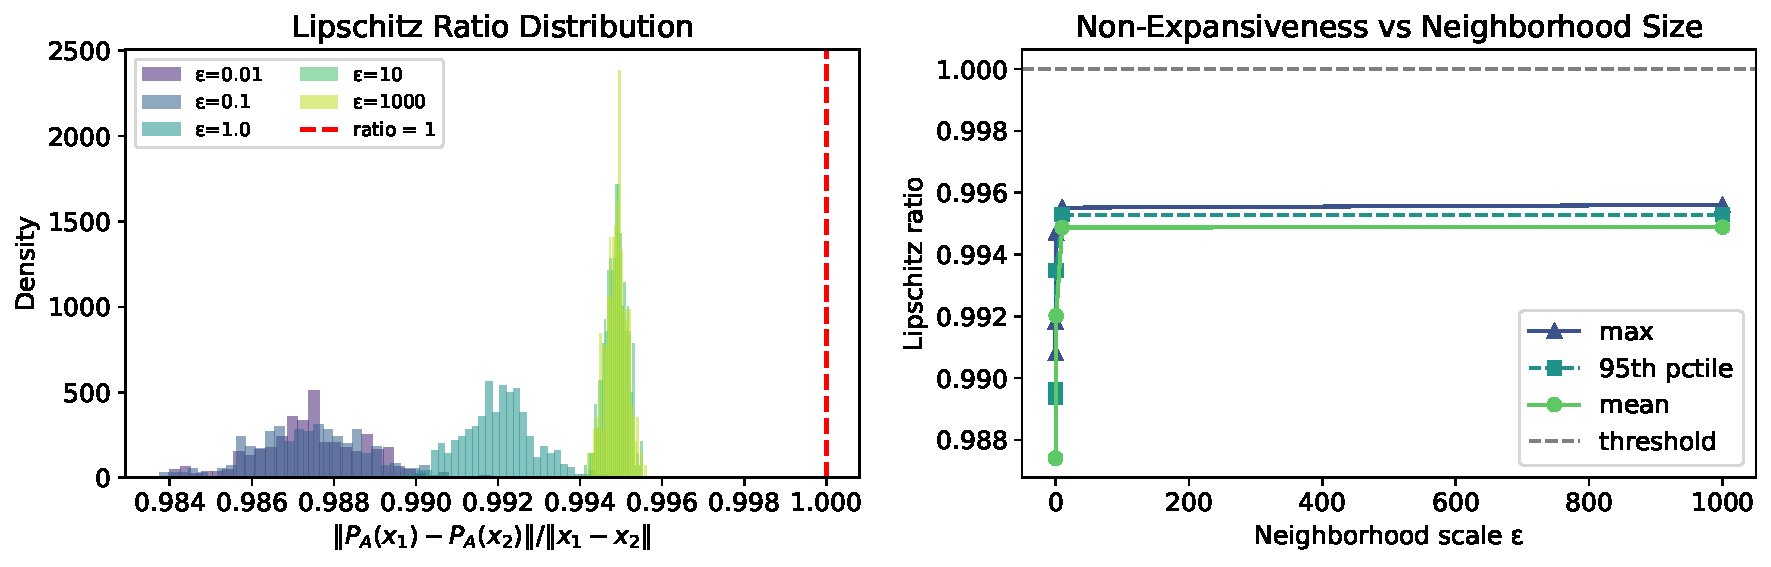
\includegraphics[width=1.0\linewidth]{images/other_benchmarks/local_nonexpansiveness_tensor_32.pdf}
    \caption{Empirical validation of local non-expansiveness for the MatMul projection on a 32x32x32 tensor. Even with an neigborhood scale of 1000, the non expansiveness remains true}
    \label{fig:nonexpansiveness_32}
\end{figure}
To validate local non-expansiveness, we manually calculate the projection distances across various disturbances to determine whether the linear layer respects this condition. Provided that the linear layer has a sufficiently large dimensionality, our experiments confirm that the local non-expansiveness property hold.

However, for tiny matrices which are atypical in deep learning applications the local non-expansiveness condition does not strictly hold:


\begin{figure}[htbp]
    \centering
    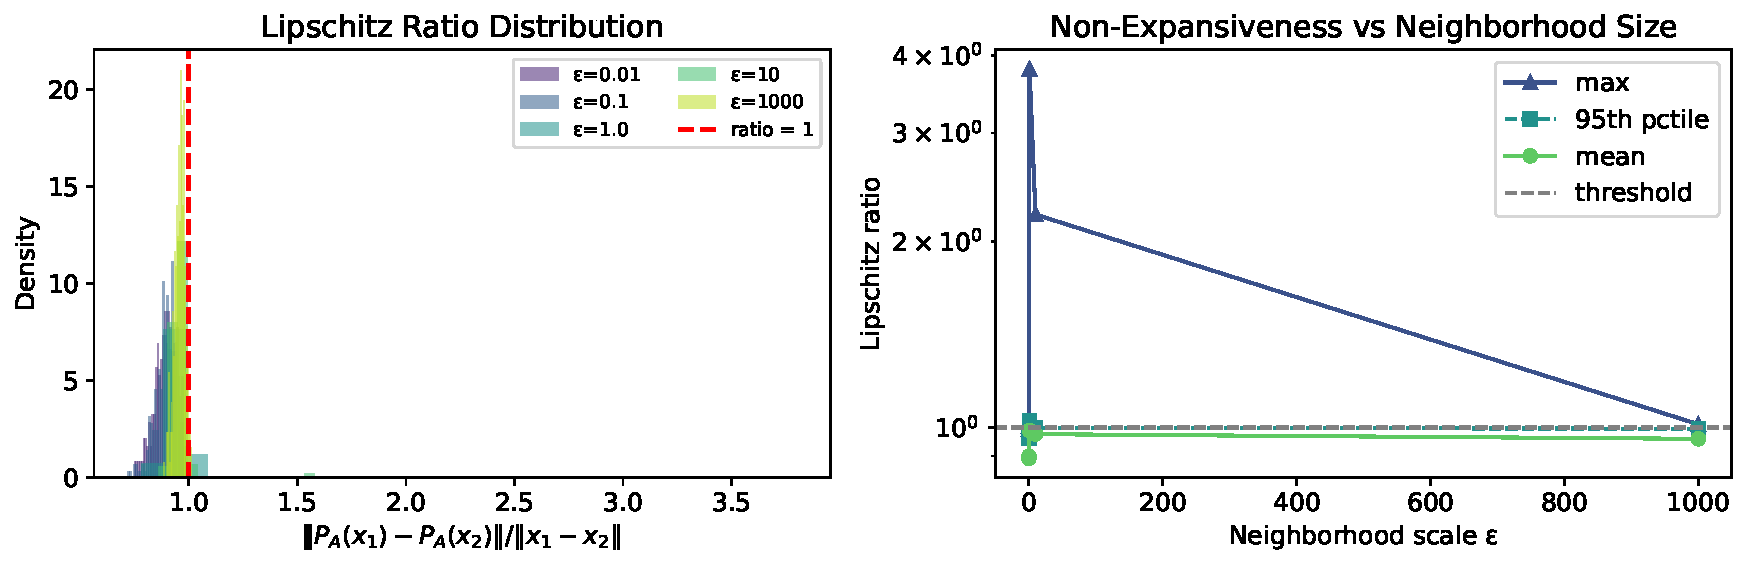
\includegraphics[width=1.0\linewidth]{images/other_benchmarks/local_nonexpansiveness_matmul_3.pdf}
    \caption{Empirical validation of local non-expansiveness for the MatMul projection on a 3x3x3 tensor. The results demonstrate that while the condition holds on average, there are outliers where it is violated.}
    \label{fig:nonexpansiveness_3}
\end{figure}

\subsection{Proof Vanishing Targets}
\label{sec:proof-vanishing-targets}
To prove the vanishing targets phenomenon, we will demonstrate by induction that the target signal magnitude at each layer is bounded by the magnitude at the succeeding layer.

We first recall the definition of the target signal magnitude at hidden layer $i$:
\begin{equation*}
\delta^{i} := \|\bar{h}^{i} - h^{i}\|_2
\end{equation*}

Furthermore, we rely on the assumption of Local Non-Expansiveness. Let the constraint set associated with layer $i+1$ be defined as:
\begin{equation*}
A_{i+1} := \{(h^{(i)}, \theta^{(i+1)}, h^{(i+1)}) \mid h^{(i+1)} = f_{i+1}(h^{(i)}, \theta^{(i+1)})\}
\end{equation*}

While $A_{i+1}$ is generally non-convex due to nonlinearities and bilinear weight-activation interactions, we assume that within a sufficiently small neighborhood of the current iterates, the projection operator $P_{A_{i+1}}$ behaves non-expansively

We proceed by induction moving backward from the output layer $N$.
\paragraph{Base case}
At the output layer $N$, the proximal update for an arbitrary loss function $\mathcal{L}$ gives

$$\bar{h}^{(N), n} \;\in\; \underset{h}{\mathrm{arg\,min}} \left( \mathcal{L}\bigl(h, y_{\mathrm{target}}^{n}\bigr) + \frac{\lambda}{2} \bigl\|h - h^{N}\bigr\|_2^2 \right).$$

Assuming $\mathcal{L}$ is proper and lower semi-continuous, this minimum is attained and bounded, so $\delta^{N} = \|\bar{h}^{N} - h^{N}\|_2 < \infty$.

\paragraph{Inductive step.}
Suppose $\delta^{i+1}$ is finite. Consider the two points in the joint space $(h^{i}, \theta^{i+1}, h^{i+1})$:
\begin{align*}
A &= \bigl(h^{i},\; \theta^{i+1},\; \bar{h}^{i+1}\bigr), \\
B &= \bigl(h^{i},\; \theta^{i+1},\; h^{i+1}\bigr).
\end{align*}

Since the forward pass satisfies the constraint exactly, $B \in A_{i+1}$ and hence $\Pi_{A_{i+1}}(B) = B$. By Assumption~\ref{ass:non-expansive}:
\[
\|\Pi_{A_{i+1}}(A) - \Pi_{A_{i+1}}(B)\|_2^2 \;\leq\; \|A - B\|_2^2
\]
Expanding both sides and using the fact that $A$ and $B$ agree in their first two components:
\[
\|\bar{h}^{(i), n} - h^{(i), n}\|_2^2 + \|\Delta \theta^{(i+1)}\|_2^2 + \| h^{(i+1), n+1} - h^{(i+1), n}\|_2^2
\;\leq\;
\|\bar{h}^{(i+1), n} - h^{(i+1), n}\|_2^2
\]
which gives $\bigl(\delta^{(i), n}\bigr)^2 \leq \bigl(\delta^{(i+1), n}\bigr)^2 - \bigl(\|\Delta \theta^{(i+1)}\|_2^2 + \|\Delta h^{(i+1)}\|_2^2\bigr) \leq \bigl(\delta^{(i+1), n}\bigr)^2$, and therefore $\delta^{(i), n} \leq \delta^{(i+1), n}$.

\section{Details Experiments}
Unless explicitly overridden in a per-experiment paragraph, all benchmarks share the configuration in
Table~\ref{tab:shared-protocol}. The exact YAML configurations underlying every figure is released alongside the code in
\texttt{experiments/\{mlp,deep,cnn\_benchmarks\}/*.yaml}; the entry
points are \texttt{bench\_ptorch.py}, \texttt{bench\_torch.py}.
\begin{table}[h]
\centering
\caption{Default experimental protocol. Per-experiment overrides
(maximum step budget, early-stopping patience, network width/depth,
loss function, projection norm, and optimizer) are stated in the
corresponding paragraphs and faithfully reflect the released YAML
configs.}
\small
\renewcommand{\arraystretch}{1.0}
\begin{tabular}{ll}
\toprule
\textbf{Component} & \textbf{Default value} \\
\midrule
Frameworks compared      & $\mathcal{P}$Torch, \texttt{pjax}~\cite{bergmeister2025projection}, \texttt{torch}~\cite{paszke2019pytorchimperativestylehighperformance} \\
Random seed              & 43 (per-run seed $= 43 + r$ for $r=0,1,2$) \\
Batch size               & 32 \\
Evaluation interval      & every 200 optimization steps on the held-out validation split \\
Train/val/test split     & 90\%/10\% of the official train set; official test set held back \\
Initialization           & PyTorch defaults (Kaiming-normal for linear/conv weights) \\
$\mathcal{P}$Torch optimizer  & \texttt{ProjectionMuon}, lr $=10^{-3}$ \\
$\mathcal{P}$Torch projection norm & $\ell_\infty$ \\
$\mathcal{P}$Torch projection scales & $\alpha = \gamma = 1$ (default) \\
$\mathcal{P}$Torch loss       & \texttt{CrossEntropy} (proximal, $\lambda=1$) \\
\texttt{pjax} optimizer  & \texttt{DouglasRachford}, 50 inner projection steps per batch (matches~\cite{bergmeister2025projection}) \\
\texttt{torch} optimizer & \texttt{Adam}, lr $=10^{-3}$, $\beta_1{=}0.9,\beta_2{=}0.999$ \\
\texttt{torch} loss      & \texttt{CrossEntropyLoss} \\
Hardware / software      & 1$\times$ NVIDIA L40S (46\,GB); 16 cores; 188\,GB RAM\\
\bottomrule
\end{tabular}
\label{tab:shared-protocol}
\end{table}
\section{Useful Projections}
\label{sec:projections}

\begin{tcolorbox}[projectioncard, title=ReLU Layer ($\ell_2$)]


\textbf{Constraint}
\[
C_{\mathrm{ReLU}} = \{(x, z) \mid z = \max(0, x)\}
\]

\textbf{Projection $\ell_2$}

Let the projection onto the inactive branch be $x_1 = \min(x, 0)$, with squared distance:
\[
d_1^2 = (x - x_1)^2 + z^2
\]
Let the projection onto the active branch be $x_2 = \max\left(\frac{x + z}{2}, 0\right)$, with squared distance:
\[
d_2^2 = (x - x_2)^2 + (z - x_2)^2
\]
The projected coordinates $(\overline{x}, \overline{z})$ are chosen by minimizing the $L_2$ distance:
\[
(\overline{x}, \overline{z}) = 
\begin{cases} 
(x_1, 0) & \text{if } d_1^2 < d_2^2 \\ 
(x_2, x_2) & \text{otherwise} 
\end{cases}
\]
\textbf{Derivation Source}
\cite{ elser2019learning}
\end{tcolorbox}

\begin{tcolorbox}[projectioncard, title=ReLU Layer ($\ell_\infty$)]
\\
\textbf{Constraint}
\[
C_{\mathrm{ReLU}} = \{(x, z) \mid z = \max(0, x)\}
\]

\textbf{Projection $\ell_\infty$}


Let the projection onto the inactive branch be $x_1 = \min(x, 0)$:
\[
d_1 = \max(|x - x_1|, |z|)
\]
Let the projection onto the active branch be $x_2 = \max\left(\frac{x + z}{2}, 0\right)$:
\[
d_2 = \max(|x - x_2|, |z - x_2|)
\]
The projected coordinates $(\overline{x}, \overline{z})$ :
\[
(\overline{x}, \overline{z}) = 
\begin{cases} 
(x_1, 0) & \text{if } d_1 < d_2 \\ 
(x_2, x_2) & \text{otherwise} 
\end{cases}
\]
\end{tcolorbox}
% -------------------------
\begin{tcolorbox}[projectioncard, title=Linear Layer]
\\
\\
\textbf{Constraint Set}
\[
C_{\mathrm{dot}} = \{(h, \theta, h^+) \mid \theta^\top h = h^+\}
\]

\textbf{Projection $\ell_2$}
\[
\begin{aligned}
\overline{h} &= \frac{h + t\,\theta}{1-t^2}, \\
\overline{\theta} &= \frac{\theta + t\,h}{1-t^2}, \\
\overline{h}^+ &= h^+ - \frac{t}{\gamma^2}
\end{aligned}
\]
\textbf{Derivation Source}
\cite{bauschke_bilinear, elser2019learning, bergmeister2025projection}
\textit{The scalar $t$ is computed via Newton's method.}
\vspace{1.0em}

\textbf{Projection $\ell_\infty$}
\[
\begin{aligned}
\overline{h}_k &= h_k + \Delta h_k, \quad |\Delta h_k| = \epsilon^* \\
\overline{\theta}_k &= \theta_k + \Delta \theta_k, \quad |\Delta \theta_k| = \epsilon^* \\
\overline{h}^+ &= h^+ + \Delta h^+, \quad |\Delta h^+| = \frac{\epsilon^*}{\gamma^2}
\end{aligned}
\]

\vspace{0.5em}
\textit{Where the optimal box radius $\epsilon^*$ is the root of $F(\epsilon) = 0$, defined as:}
\[
F(\epsilon) = \sum_{k=1}^{n} M_k(\epsilon) + \frac{\epsilon}{\gamma^2} - |h^{+} - \theta^\top h|
\]
\[
M_k(\epsilon) = m_k(\epsilon)\bigl(a_k\epsilon+\epsilon^2\bigr) + \bigl(1-m_k(\epsilon)\bigr)\bigl(b_k\epsilon-\epsilon^2\bigr)
\]
\end{tcolorbox}

\paragraph{$\ell_2$ derivation}
As \cref{sec:matmul} builds up on a weighted version of this derivation, the full derivation is placed below for the linear layer constraint in l2 using lagrangian multipliers as in \cite{elser2019learning}.
\begin{equation}
  \label{eq:constraint-dot}
  C_{\mathrm{dot}} := \{(h, \theta, h^+)\in \mathbb{R}^n \times \mathbb{R}^n \times \mathbb{R} \mid \theta^\top h = h^+\}.
\end{equation}
So we are searching for the closest point in the feasibility set under a weighted distance norm:
\[
\Pi_{C_{\mathrm{dot}}}^{\alpha, \gamma}(h, \theta, h^+) \in \operatorname*{arg\,min}_{(\overline{h}, \overline{\theta}, \overline{h}^+) \in C_{\mathrm{dot}}} \left( \lVert \overline{h}-h \rVert^2 + \alpha\lVert \overline{\theta}-\theta \rVert^2 + \gamma^2(\overline{h}^+ - h^+)^2 \right).
\]

Given a current iterate $(h, \theta, h^+)$ and scaling parameters $\alpha, \gamma>0$, the projection is
\begin{equation}
  \label{eq:proj-bilinear-layer}
  \begin{aligned}
    \min_{\overline{h}^+\in\mathbb{R},\,\overline{h},\overline{\theta}\in\mathbb{R}^n}\; &\ \lVert \overline{h}-h\rVert^2 + \alpha\lVert \overline{\theta}-\theta\rVert^2 + \gamma^2\,(\overline{h}^+-h^+)^2\\
    \text{s.t. } &\ \overline{h}^+ = \overline{\theta}^\top \overline{h}.
  \end{aligned}
\end{equation}
Introduce a Lagrangian multiplier $\lambda$ and define
\[
  \mathcal{L} = \lVert \overline{h}-h\rVert^2 + \alpha\lVert \overline{\theta}-\theta\rVert^2 + \gamma^2(\overline{h}^+-h^+)^2 + \lambda\,(\overline{h}^+ - \overline{\theta}^\top \overline{h}).
\]
Setting $\nabla \mathcal{L} = 0$ and using $t:=\lambda/2$ yields
\[
  \overline{h} = h + t\,\overline{\theta},\qquad \overline{\theta} = \theta + \frac{t}{\alpha}\,\overline{h},\qquad \overline{h}^+ = h^+ - \frac{t}{\gamma^2}.
\]
Solving the coupled system gives
\[
  \overline{h} = \frac{\alpha}{\alpha-t^2}(h + t\,\theta),\qquad \overline{\theta} = \frac{\alpha\theta }{\alpha-t^2} +  \frac{t\,h}{\alpha-t^2} .
\]
Substituting into the constraint $\overline{h}^+=\overline{\theta}^\top \overline{h}$ leads to a scalar equation $f(t)=0$:
\[
  h^+ - \frac{t}{\gamma^2} 
  = \frac{(\alpha\theta+t h)^\top \alpha(h+t \theta)}{(\alpha-t^2)^2} 
  = \alpha \frac{p(\alpha+t^2)+q t}{(\alpha-t^2)^2},
\]
where $p:=\theta^\top h$ and $q:=\lVert h\rVert^2 + \alpha\lVert \theta\rVert^2$.
The root can be found efficiently with Newton's method, after which $\overline{h}, \overline{\theta}, \overline{h}^+$ are reconstructed from the expressions above.

\paragraph{$\ell_\infty$ derivation}
\label{sec:bilinear-inf}
\label{sec:linf}
The optimization geometry of the projection step can be modified to achieve
different training properties. We replace the standard Euclidean projection with
the $\ell_\infty$ one.

Given the current state $(h, \theta, h^{+}) \in \mathbb{R}^n \times \mathbb{R}^n \times
\mathbb{R}$ and a scaling parameter $\gamma > 0$, the $\ell_\infty$ bilinear
projection problem is
\begin{equation}
\min_{\bar{h}, \bar{\theta}, \bar{h}^+} \| (\bar{h}, \bar{\theta}, \gamma^2 \bar{h}^+) - (h, \theta, \gamma^2 h^+) \|_\infty \quad \text{s.t.} \quad \bar{\theta}^\top \bar{h} = \bar{h}^+
\end{equation}
\\
The key is finding the smallest feasible box radius $\epsilon^* \geq 0$ such
that all constraints are simultaneously satisfiable. Let $\Delta h = \bar h - h$ and $\Delta \theta = \bar \theta - \theta$. The
constraints read
\[
  |\Delta h_k| \leq \epsilon \quad |\Delta \theta_{k}| \leq \epsilon
  \quad (k=1,\dots,n) 
  \qquad |\bar h^{+} - h^{+}| \leq \frac{\epsilon}{\gamma^2}.
\]
The total dot-product change decomposes coordinate-wise. Let $D = \theta^\top h$ and $\bar{D} = \bar{\theta}^\top \bar{h}$:
\begin{equation}
\label{eq:bilinf-DeltaP}
\begin{aligned}
 \bar{D} &= (\theta + \Delta \theta)^\top (h + \Delta h) \\
  \Delta D_k 
    \;&=\; (h_k+\Delta h_k)(\theta_{k}+\Delta \theta_{k}) - h_k \theta_{k} \\
    \;&=\; h_k\,\Delta \theta_{k} + \theta_{k}\,\Delta h_k + \Delta h_k\,\Delta \theta_{k}.
\end{aligned}
\end{equation}

\begin{figure}[htbp]
    \centering
    % Left side: The Table
    \begin{minipage}{0.4\textwidth}

    

        \renewcommand{\arraystretch}{1.35}
        \begin{tabular}{ccc}
        \hline
        $\Delta h_k$ & $\Delta \theta_{k}$ & $\Delta D_k$ \\
        \hline
        $+\epsilon$ & $+\epsilon$ & $\phantom{-}\epsilon(h_k+\theta_{k})+\epsilon^2$ \\
        $-\epsilon$ & $-\epsilon$ & $-\epsilon(h_k+\theta_{k})+\epsilon^2$ \\
        \hline
        $+\epsilon$ & $-\epsilon$ & $\phantom{-}\epsilon(\theta_{k}-h_k)-\epsilon^2$ \\
        $-\epsilon$ & $+\epsilon$ & $\phantom{-}\epsilon(h_k-\theta_{k})-\epsilon^2$ \\
        \hline
        \end{tabular}
    \end{minipage}\hfill
    % Right side: The Figure
    \begin{minipage}{0.6\textwidth}
        \centering
        \providecolor{KUL-BLUE}{RGB}{29, 55, 104}
\providecolor{KUL-ORANGE}{RGB}{230, 140, 0}

\begin{tikzpicture}[>=stealth,every node/.style={font=\small},scale=0.5]
  % axes
  \draw[thin,->,black!55] (-3.3,0)--(3.5,0) node[right,text=black]{$\Delta h_k$};
  \draw[thin,->,black!55] (0,-3.3)--(0,3.5) node[above,text=black]{$\Delta \theta_{k}$};
  
  % box (matching the 'op' style fill and draw colors from KUL)
  \fill[black!8] (-2.4,-2.4) rectangle (2.4,2.4);
  \draw[thick,black!65] (-2.4,-2.4) rectangle (2.4,2.4);

  % tick marks
  \foreach \v/\l in {3/{$+\epsilon$},-3/{$-\epsilon$}}{
    \draw[black!65] (\v,2pt)--(\v,-2pt) node[below,yshift=-2pt,text=black]{\l};
    \draw[black!65] (2pt,\v)--(-2pt,\v) node[left,xshift=-2pt,text=black]{\l};
  }

  % --- same-sign pair (KUL-BLUE) ---
  \fill[KUL-BLUE!85!black] (2.4,2.4) circle (4pt);
  \fill[KUL-BLUE!85!black] (-2.4,-2.4) circle (4pt);

  \node[KUL-BLUE!85!black,anchor=south west,align=left] at (2.5,2.3)
    {$\epsilon(h_k+\theta_{k})+\epsilon^2$};
  \node[KUL-BLUE!85!black,anchor=north east,align=right] at (-2.5,-2.3)
    {$-\epsilon(h_k+\theta_{k})+\epsilon^2$};

  % dashed line connecting same-sign pair
  \draw[KUL-BLUE!85!black,dashed,thick] (2.4,2.4)--(-2.4,-2.4);

  % --- opposite-sign pair (KUL-ORANGE) ---
  \fill[KUL-ORANGE!85!black] (2.4,-2.4) circle (4pt);
  \fill[KUL-ORANGE!85!black] (-2.4,2.4) circle (4pt);

  \node[KUL-ORANGE!85!black,anchor=north west,align=left] at (2.5,-2.3)
    {$\epsilon(\theta_{k}-h_k)-\epsilon^2$};
  \node[KUL-ORANGE!85!black,anchor=south east,align=right] at (-2.5,2.3)
    {$\epsilon(h_k-\theta_{k})-\epsilon^2$};

  % dashed line connecting opposite-sign pair
  \draw[KUL-ORANGE!85!black,dashed,thick] (2.4,-2.4)--(-2.4,2.4);

\end{tikzpicture}
        \vspace{-1.0pt}
        \caption{Graphical interpretation of $\Delta D_k$}
    \end{minipage}
\end{figure}
The maximum upward contribution of coordinate $k$ to the dot product is
\begin{equation}
\label{eq:bilinf-Mk}
  M_k(\epsilon)
    \;=\; \max\!\Bigl(
      \epsilon|h_k+\theta_{k}|+\epsilon^2,\;
      \epsilon|h_k-\theta_{k}|-\epsilon^2
    \Bigr).
\end{equation}

In the case $D=\theta^\top h < h^{+}$, the smallest feasible radius $\epsilon^*$ is
the unique positive root of
\begin{equation}
\label{eq:bilinf-root}
\begin{aligned}
    D+\sum_{k=1}^{n} M_k(\epsilon)
      &= h^{+}  - \frac{\epsilon}{\gamma^2}, \\
    F(\epsilon)
      &= \sum_{k=1}^{n} M_k(\epsilon) + \frac{\epsilon}{\gamma^2} - (h^{+} - D)
      \;=\; 0.
\end{aligned}
\end{equation}
$F$ is continuous, strictly monotone increasing, and piecewise quadratic
in $\epsilon$.

Each coordinate contributes at most one kink to $F$, occurring at
\[
  \epsilon_k^{\mathrm{kink}}
    \;=\; \max\!\left\{0,\;
      \frac{|h_k-\theta_{k}|-|h_k+\theta_{k}|}{2}
    \right\}.
\]

Sorting these kink points requires $\mathcal{O}(n\log n)$ time, with root
evaluation linear in $n$ on each interval.
\paragraph{$\mathcal{O}(n)$ Solve via Branch Masking}
Geometrically, defining $a_k := |h_k+\theta_k|$ and $b_k := |h_k-\theta_k|$ corresponds to a $45^{\circ}$ coordinate rotation of the $(h_k, \theta_k)$ plane. This rotation decouples the bilinear product into independent axes, aligning the analysis naturally with the diagonals of the $l_\infty$ bounding box. Coordinate $k$ contributes via whichever of two geometrically distinct regimes yields the larger reach. In the same-sign branch ($a_k\epsilon + \epsilon^2$), the box pushes $h_k$ and $\theta_k$ in the same direction, expanding their sum. This regime dominates when $\epsilon$ is large relative to the gap $b_k - a_k$. Conversely, in the opp-sign branch ($b_k\epsilon - \epsilon^2$), the box pushes $h_k$ and $\theta_k$ in opposite directions, collapsing their difference. This branch dominates when $\epsilon$ is small.

The crossover between these branches occurs at the unique kink $\epsilon_k^{\mathrm{kink}} = \max\{0, (b_k - a_k)/2\}$. For values of $\epsilon$ above this threshold, the same-sign branch wins; below it, the opp-sign branch wins. This switching behavior is encoded by the binary mask
\[
  m_k(\epsilon) \;:=\; \mathbf{1}\!\left[2\epsilon \geq b_k - a_k\right],
\]
so that the per-coordinate reach takes the \emph{unified} branch-free form
\begin{equation}
  M_k(\epsilon)
    \;=\; m_k(\epsilon)\bigl(a_k\epsilon+\epsilon^2\bigr)
      + \bigl(1-m_k(\epsilon)\bigr)\bigl(b_k\epsilon-\epsilon^2\bigr).
\end{equation}

Since $m_k(\epsilon)$ is a step function that flips \emph{at most once} as
$\epsilon$ increases, both $F(\epsilon)$ and its derivative
\begin{equation}
  F'(\epsilon)
    \;=\; \sum_{k=1}^{n}\Bigl[
        m_k(\epsilon)\bigl(a_k + 2\epsilon\bigr)
      + \bigl(1-m_k(\epsilon)\bigr)\bigl(b_k - 2\epsilon\bigr)
    \Bigr] + \frac{1}{\gamma^2}
\end{equation}
are computable in a single $\mathcal{O}(n)$ pass by evaluating both branch
expressions and selecting via $m_k$, \emph{without sorting or branching in
control flow}. The safeguarded
iteration
\[
  \epsilon_{t+1}
    \;=\; \max\!\left(\ell_t,\min\!\left(r_t, \epsilon_t - \frac{F(\epsilon_t)}{F'(\epsilon_t)}\right)\right)
\]
Converges in $\mathcal{O}(1)$ iterations in practice: the piecewise-quadratic means each Newton step either lands in the correct segment immediately, or crosses at most one kink before the next iterate is already in the final segment. The full solve is therefore $\mathcal{O}(n)$.


\IfFileExists{checklist.tex}{\input{checklist.tex}}{}

\end{document}
 